% Options for packages loaded elsewhere
\PassOptionsToPackage{unicode}{hyperref}
\PassOptionsToPackage{hyphens}{url}
\PassOptionsToPackage{dvipsnames,svgnames,x11names}{xcolor}
%
\documentclass[
  11,
  a4paper,
]{article}

\usepackage{amsmath,amssymb}
\usepackage{setspace}
\usepackage{iftex}
\ifPDFTeX
  \usepackage[T1]{fontenc}
  \usepackage[utf8]{inputenc}
  \usepackage{textcomp} % provide euro and other symbols
\else % if luatex or xetex
  \usepackage{unicode-math}
  \defaultfontfeatures{Scale=MatchLowercase}
  \defaultfontfeatures[\rmfamily]{Ligatures=TeX,Scale=1}
\fi
\usepackage{lmodern}
\ifPDFTeX\else  
    % xetex/luatex font selection
  \setmainfont[Numbers=Lowercase,Numbers=Proportional]{Times New Roman}
\fi
% Use upquote if available, for straight quotes in verbatim environments
\IfFileExists{upquote.sty}{\usepackage{upquote}}{}
\IfFileExists{microtype.sty}{% use microtype if available
  \usepackage[]{microtype}
  \UseMicrotypeSet[protrusion]{basicmath} % disable protrusion for tt fonts
}{}
\makeatletter
\@ifundefined{KOMAClassName}{% if non-KOMA class
  \IfFileExists{parskip.sty}{%
    \usepackage{parskip}
  }{% else
    \setlength{\parindent}{0pt}
    \setlength{\parskip}{6pt plus 2pt minus 1pt}}
}{% if KOMA class
  \KOMAoptions{parskip=half}}
\makeatother
\usepackage{xcolor}
\usepackage[top=15mm,left=22.5mm,right=22.5mm,bottom=15mm]{geometry}
\setlength{\emergencystretch}{3em} % prevent overfull lines
\setcounter{secnumdepth}{-\maxdimen} % remove section numbering
% Make \paragraph and \subparagraph free-standing
\ifx\paragraph\undefined\else
  \let\oldparagraph\paragraph
  \renewcommand{\paragraph}[1]{\oldparagraph{#1}\mbox{}}
\fi
\ifx\subparagraph\undefined\else
  \let\oldsubparagraph\subparagraph
  \renewcommand{\subparagraph}[1]{\oldsubparagraph{#1}\mbox{}}
\fi


\providecommand{\tightlist}{%
  \setlength{\itemsep}{0pt}\setlength{\parskip}{0pt}}\usepackage{longtable,booktabs,array}
\usepackage{calc} % for calculating minipage widths
% Correct order of tables after \paragraph or \subparagraph
\usepackage{etoolbox}
\makeatletter
\patchcmd\longtable{\par}{\if@noskipsec\mbox{}\fi\par}{}{}
\makeatother
% Allow footnotes in longtable head/foot
\IfFileExists{footnotehyper.sty}{\usepackage{footnotehyper}}{\usepackage{footnote}}
\makesavenoteenv{longtable}
\usepackage{graphicx}
\makeatletter
\def\maxwidth{\ifdim\Gin@nat@width>\linewidth\linewidth\else\Gin@nat@width\fi}
\def\maxheight{\ifdim\Gin@nat@height>\textheight\textheight\else\Gin@nat@height\fi}
\makeatother
% Scale images if necessary, so that they will not overflow the page
% margins by default, and it is still possible to overwrite the defaults
% using explicit options in \includegraphics[width, height, ...]{}
\setkeys{Gin}{width=\maxwidth,height=\maxheight,keepaspectratio}
% Set default figure placement to htbp
\makeatletter
\def\fps@figure{htbp}
\makeatother
\newlength{\cslhangindent}
\setlength{\cslhangindent}{1.5em}
\newlength{\csllabelwidth}
\setlength{\csllabelwidth}{3em}
\newlength{\cslentryspacingunit} % times entry-spacing
\setlength{\cslentryspacingunit}{\parskip}
\newenvironment{CSLReferences}[2] % #1 hanging-ident, #2 entry spacing
 {% don't indent paragraphs
  \setlength{\parindent}{0pt}
  % turn on hanging indent if param 1 is 1
  \ifodd #1
  \let\oldpar\par
  \def\par{\hangindent=\cslhangindent\oldpar}
  \fi
  % set entry spacing
  \setlength{\parskip}{#2\cslentryspacingunit}
 }%
 {}
\usepackage{calc}
\newcommand{\CSLBlock}[1]{#1\hfill\break}
\newcommand{\CSLLeftMargin}[1]{\parbox[t]{\csllabelwidth}{#1}}
\newcommand{\CSLRightInline}[1]{\parbox[t]{\linewidth - \csllabelwidth}{#1}\break}
\newcommand{\CSLIndent}[1]{\hspace{\cslhangindent}#1}

\usepackage{lscape}
\newcommand{\blandscape}{\begin{landscape}}
\newcommand{\elandscape}{\end{landscape}}
\pagenumbering{roman}
\makeatletter
\makeatother
\makeatletter
\makeatother
\makeatletter
\@ifpackageloaded{caption}{}{\usepackage{caption}}
\AtBeginDocument{%
\ifdefined\contentsname
  \renewcommand*\contentsname{Table of contents}
\else
  \newcommand\contentsname{Table of contents}
\fi
\ifdefined\listfigurename
  \renewcommand*\listfigurename{List of Figures}
\else
  \newcommand\listfigurename{List of Figures}
\fi
\ifdefined\listtablename
  \renewcommand*\listtablename{List of Tables}
\else
  \newcommand\listtablename{List of Tables}
\fi
\ifdefined\figurename
  \renewcommand*\figurename{Figure}
\else
  \newcommand\figurename{Figure}
\fi
\ifdefined\tablename
  \renewcommand*\tablename{Table}
\else
  \newcommand\tablename{Table}
\fi
}
\@ifpackageloaded{float}{}{\usepackage{float}}
\floatstyle{ruled}
\@ifundefined{c@chapter}{\newfloat{codelisting}{h}{lop}}{\newfloat{codelisting}{h}{lop}[chapter]}
\floatname{codelisting}{Listing}
\newcommand*\listoflistings{\listof{codelisting}{List of Listings}}
\makeatother
\makeatletter
\@ifpackageloaded{caption}{}{\usepackage{caption}}
\@ifpackageloaded{subcaption}{}{\usepackage{subcaption}}
\makeatother
\makeatletter
\@ifpackageloaded{tcolorbox}{}{\usepackage[skins,breakable]{tcolorbox}}
\makeatother
\makeatletter
\@ifundefined{shadecolor}{\definecolor{shadecolor}{rgb}{.97, .97, .97}}
\makeatother
\makeatletter
\makeatother
\makeatletter
\makeatother
\ifLuaTeX
  \usepackage{selnolig}  % disable illegal ligatures
\fi
\IfFileExists{bookmark.sty}{\usepackage{bookmark}}{\usepackage{hyperref}}
\IfFileExists{xurl.sty}{\usepackage{xurl}}{} % add URL line breaks if available
\urlstyle{same} % disable monospaced font for URLs
\hypersetup{
  pdftitle={The genomic landscape of Acute Respiratory Distress Syndrome: a meta-analysis by information content of whole-genome studies of the host response.},
  colorlinks=true,
  linkcolor={blue},
  filecolor={Maroon},
  citecolor={Blue},
  urlcolor={Blue},
  pdfcreator={LaTeX via pandoc}}

\title{The genomic landscape of Acute Respiratory Distress Syndrome: a
meta-analysis by information content of whole-genome studies of the host
response.}
\author{}
\date{}

\begin{document}
\maketitle
\ifdefined\Shaded\renewenvironment{Shaded}{\begin{tcolorbox}[breakable, borderline west={3pt}{0pt}{shadecolor}, interior hidden, enhanced, sharp corners, boxrule=0pt, frame hidden]}{\end{tcolorbox}}\fi

\setstretch{1.5}
\begin{center}

\textbf{\LARGE Supplementary Material}

\end{center}

\newpage

\hypertarget{supplementary-methods}{%
\subsection{Supplementary Methods}\label{supplementary-methods}}

Search strategy

Inclusion criteria

\newpage

\hypertarget{search-strategy}{%
\subsubsection{Search Strategy}\label{search-strategy}}

We used the following strategy to search MEDLINE and a direct
translation to search Embase.

\textbf{1} exp Respiratory Distress Syndrome, Adult/

\textbf{2} ``acute lung injury*``.ti,ab,kf,kw

\textbf{3} 1 OR 2

\textbf{4} ``gene*``.mp

\textbf{5} ``genome*``.mp

\textbf{6} ``transcript*``.mp

\textbf{7} ``protein*``.mp

\textbf{8} 4 OR 5 OR 6 OR 7

\textbf{9} 3 AND 8

\textbf{10} (``COVID-19*'' OR ``COVID19*'' OR ``COVID-2019*'' OR
``covid'').ti,ab,kf,kw

\textbf{11} (``SARS-CoV-2*'' OR ``SARSCov-2*'' OR ``SARSCoV2*'' OR
``SARS-CoV2'').ti,sh,kf,kw

\textbf{12} (``2019-nCoV*'' OR ``2019nCoV*'' OR ``19- nCoV*'' OR
``19nCoV*'' OR ``nCoV2019*'' OR ``nCoV-2019*'' OR ``nCoV19*'' OR ``nCoV-
19*``).ti,ab,kf,kw

\textbf{13} 10 OR 11 OR 12

\textbf{14} 9 NOT 13

\textbf{15} Letter.pt OR Conference Abstract.pt OR Conference Paper.pt
OR Conference Review.pt OR Editorial.pt OR Erratum.pt OR Review.pt OR
Note.pt OR Tombstone.pt

\textbf{16} 14 NOT 15

\textbf{17} exp *adolescence/ or exp *adolescent/ or exp *child/ or exp
*childhood disease/ or exp *infant disease/ or (adolescen* or babies or
baby or boy? or boyfriend or boyhood or girlfriend or girlhood or child
or child* or child*3 or children* or girl? or infan* or juvenil* or
juvenile* or kid? or minors or minors* or neonat* or neo-nat* or
newborn* or new-born* or paediatric* or peadiatric* or pediatric* or
perinat* or preschool* or puber* or pubescen* or school* or teen* or
toddler? or underage? or under-age? or youth*).ti,kw

\textbf{18} 16 NOT 17

\textbf{19} ((exp animal/ or nonhuman/) NOT exp human/)

\textbf{20} 18 NOT 19

\textbf{21} limit 20 to yr=``1967-Current''

\newpage

\hypertarget{inclusion-criteria}{%
\subsubsection{Inclusion criteria}\label{inclusion-criteria}}

Inclusion:

\begin{itemize}
\tightlist
\item
  Human studies: \emph{in-vivo} or \emph{in-vitro}
\item
  Adults (age ≥ 18 years)
\item
  Acute Respiratory Distress Syndrome (ARDS)

  \begin{itemize}
  \tightlist
  \item
    by any contemporaneous definition
  \end{itemize}
\item
  Accepted methodologies:

  \begin{itemize}
  \tightlist
  \item
    CRISPR screen
  \item
    RNAi screen
  \item
    Protein-protein interaction study
  \item
    Host proteins incorporated into virion or virus-like particle
  \item
    Genome wide association study
  \item
    Transcriptomic study
  \item
    Proteomic study
  \end{itemize}
\end{itemize}

Exclusion:

\begin{itemize}
\tightlist
\item
  Children (age \textless{} 18 years)
\item
  Animal studies
\item
  Meta-analyses, \emph{in-silico} analyses, or re-analysis of previously
  published data
\item
  Excluded methodologies:

  \begin{itemize}
  \tightlist
  \item
    \emph{In-vitro} human studies simulating ARDS
  \item
    Candidate \emph{in-vivo} or \emph{in-vitro} transcriptomic or
    proteomic studies (defined as those investigating \textless{} 50
    genes)
  \item
    Candidate gene association studies
  \item
    Studies including fewer than 5 individuals in either the control or
    ARDS arm
  \end{itemize}
\end{itemize}

\newpage

\hypertarget{supplementary-results}{%
\subsection{Supplementary Results}\label{supplementary-results}}

Supplementary Figures 1-7

Supplementary Tables 1-4

\begin{figure}

{\centering 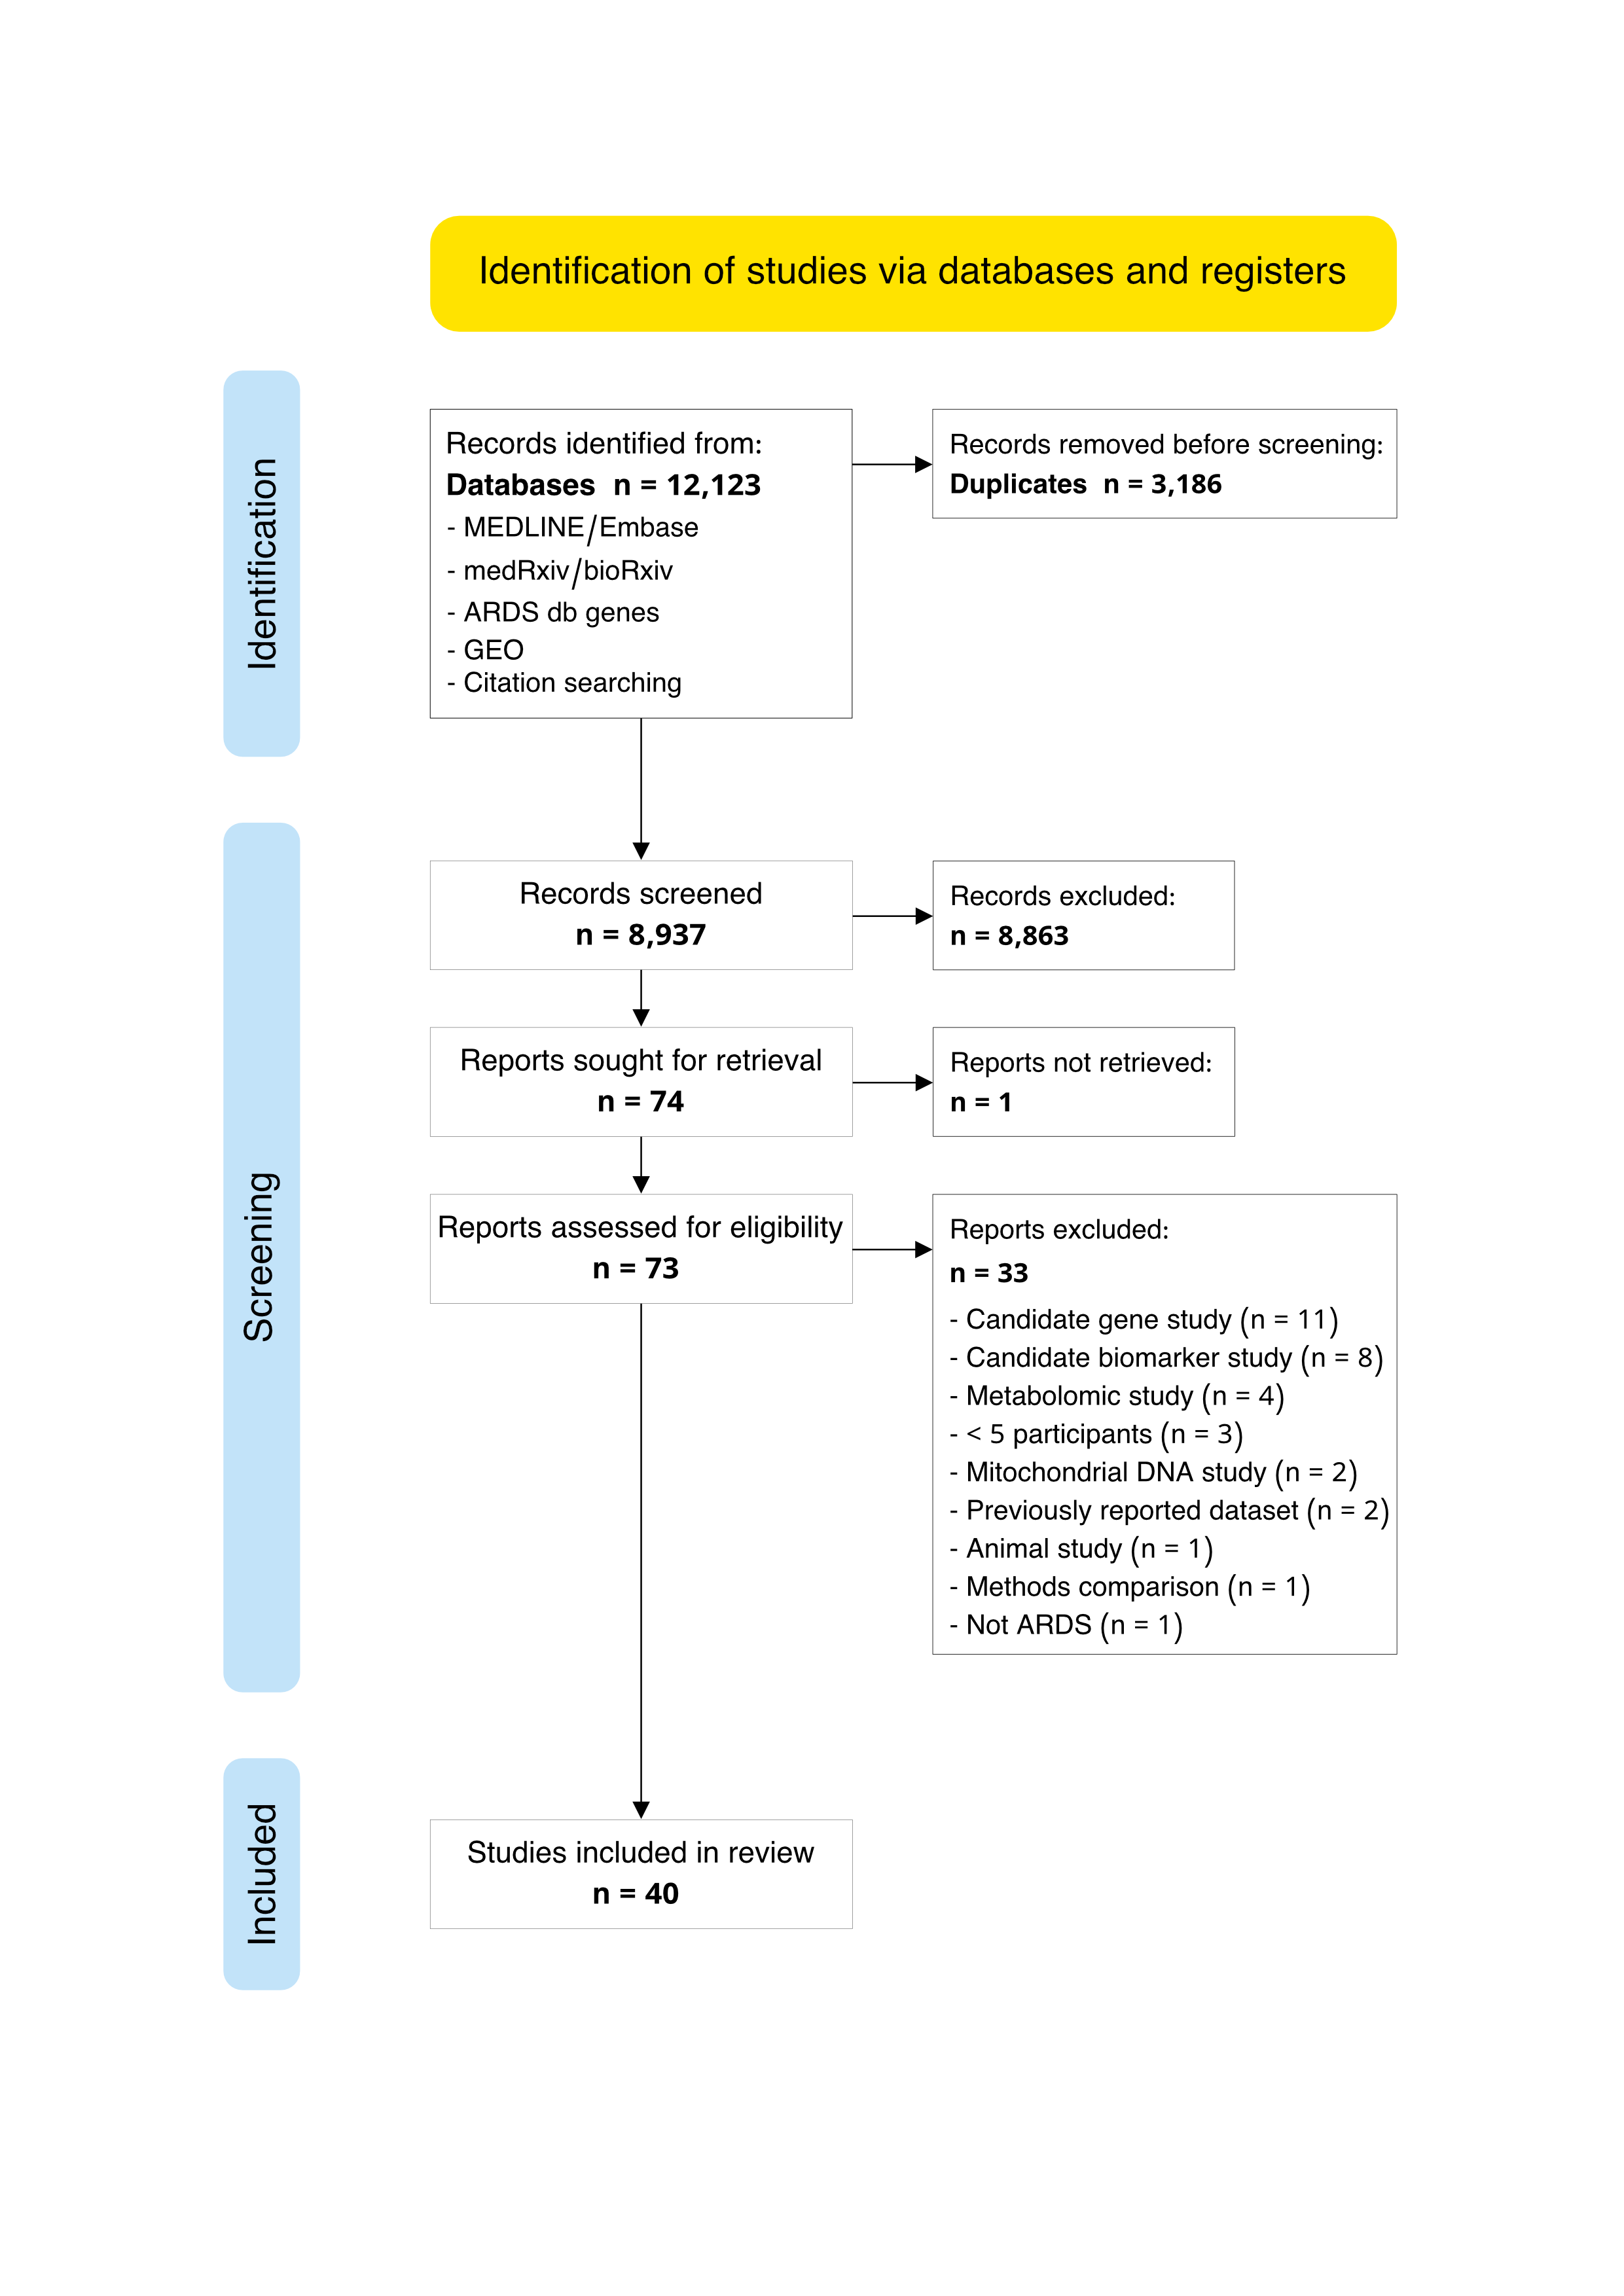
\includegraphics{../img/Supplementary_Figure_1.png}

}

\caption{\textbf{Systematic review inclusion diagram}. Abbreviations: db
- data base; GEO - NCBI Gene Expression Omnibus.}

\end{figure}

\begin{figure}

{\centering 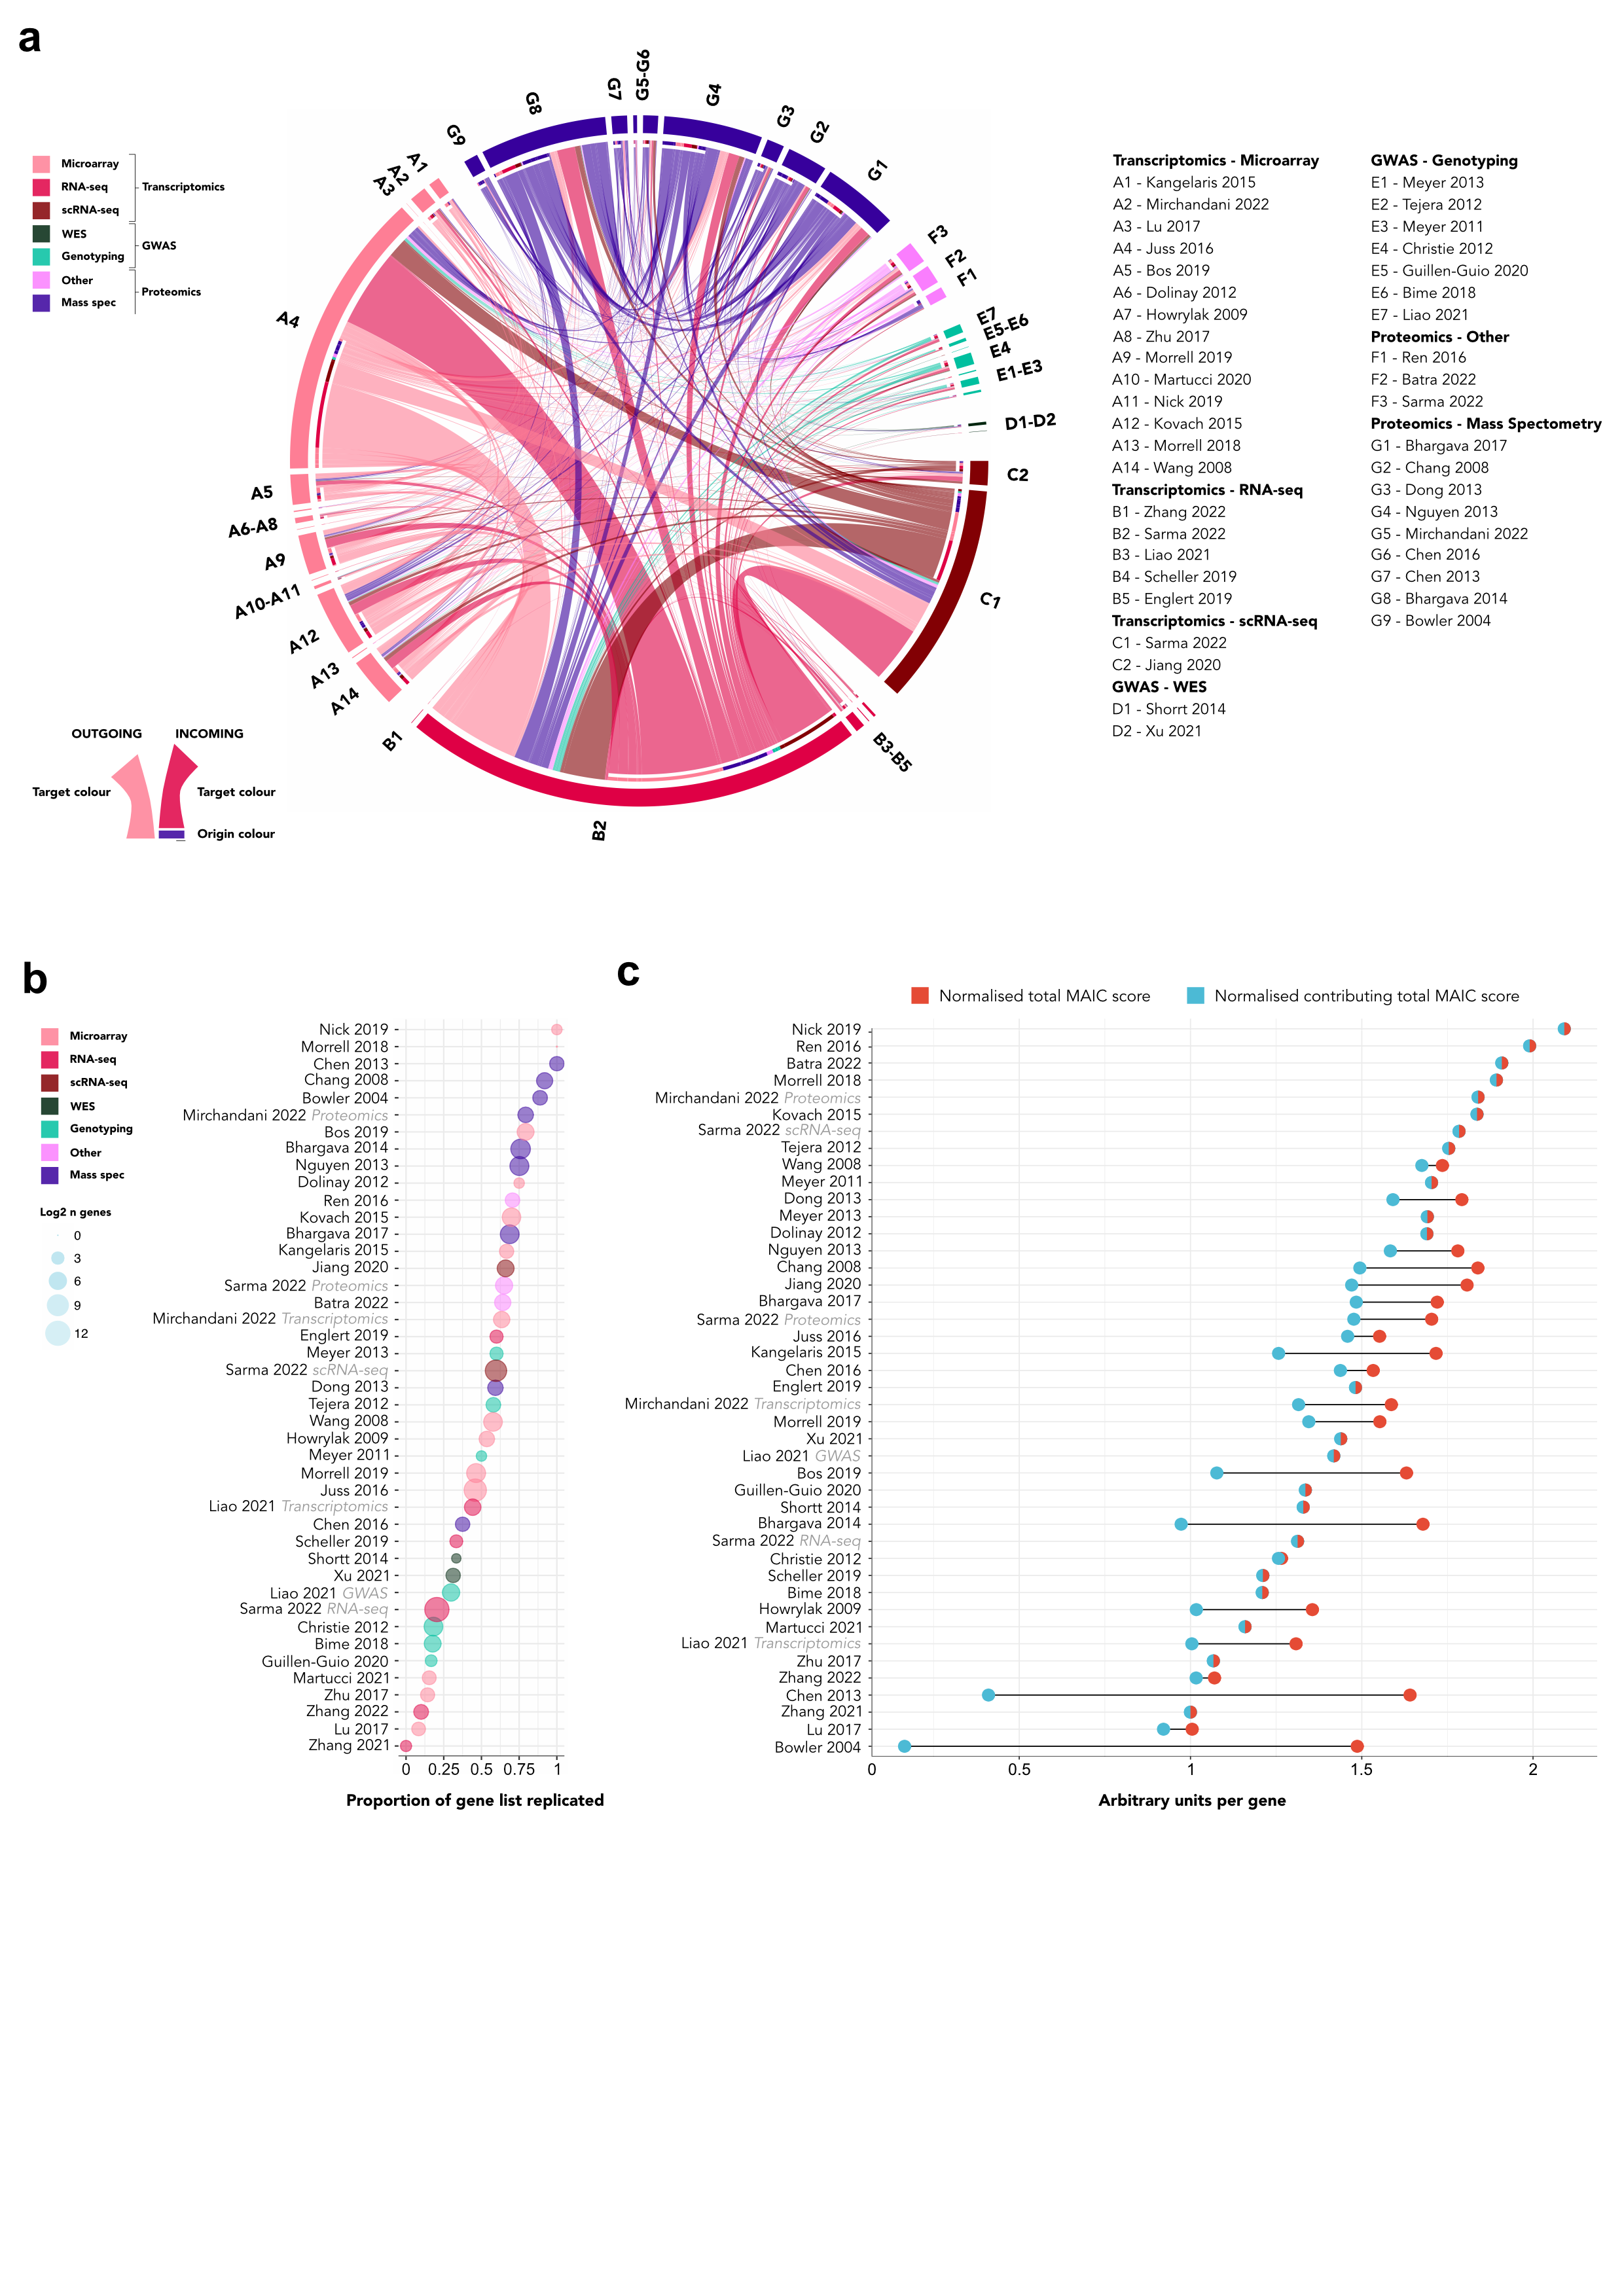
\includegraphics{../img/Supplementary_Figure_2.png}

}

\caption{\textbf{Overlap between ARDS MAIC and ARDS-associated genes and
ARDS MAIC and COVID-19 MAIC}. (a) Eular diagram of gene overlap between
ARDS MAIC and a BioLitMine search using the ARDS MeSH term. (b)
Schematic overview of a co-expression search for genes identified in the
BioLitMine search but not present in ARDS MAIC and a stacked bar plot of
the proportion of the 100 most co-expressed genes of this group and ARDS
MAIC. (c) Eular diagram of gene overlap between ARDS MAIC and the ARDS
Database of Genes. (d) Eular diagram of gene overlap between ARDS MAIC
and a MAIC of COVID-19 host-response studies. (e) Heatmap of the 50 top
ranked ARDS MAIC genes also prioritised by the COVID-19 MAIC, displaying
the ARDS MAIC score for each gene, highest gene score in each category,
and the number of supporting gene lists.}

\end{figure}

\begin{figure}

{\centering 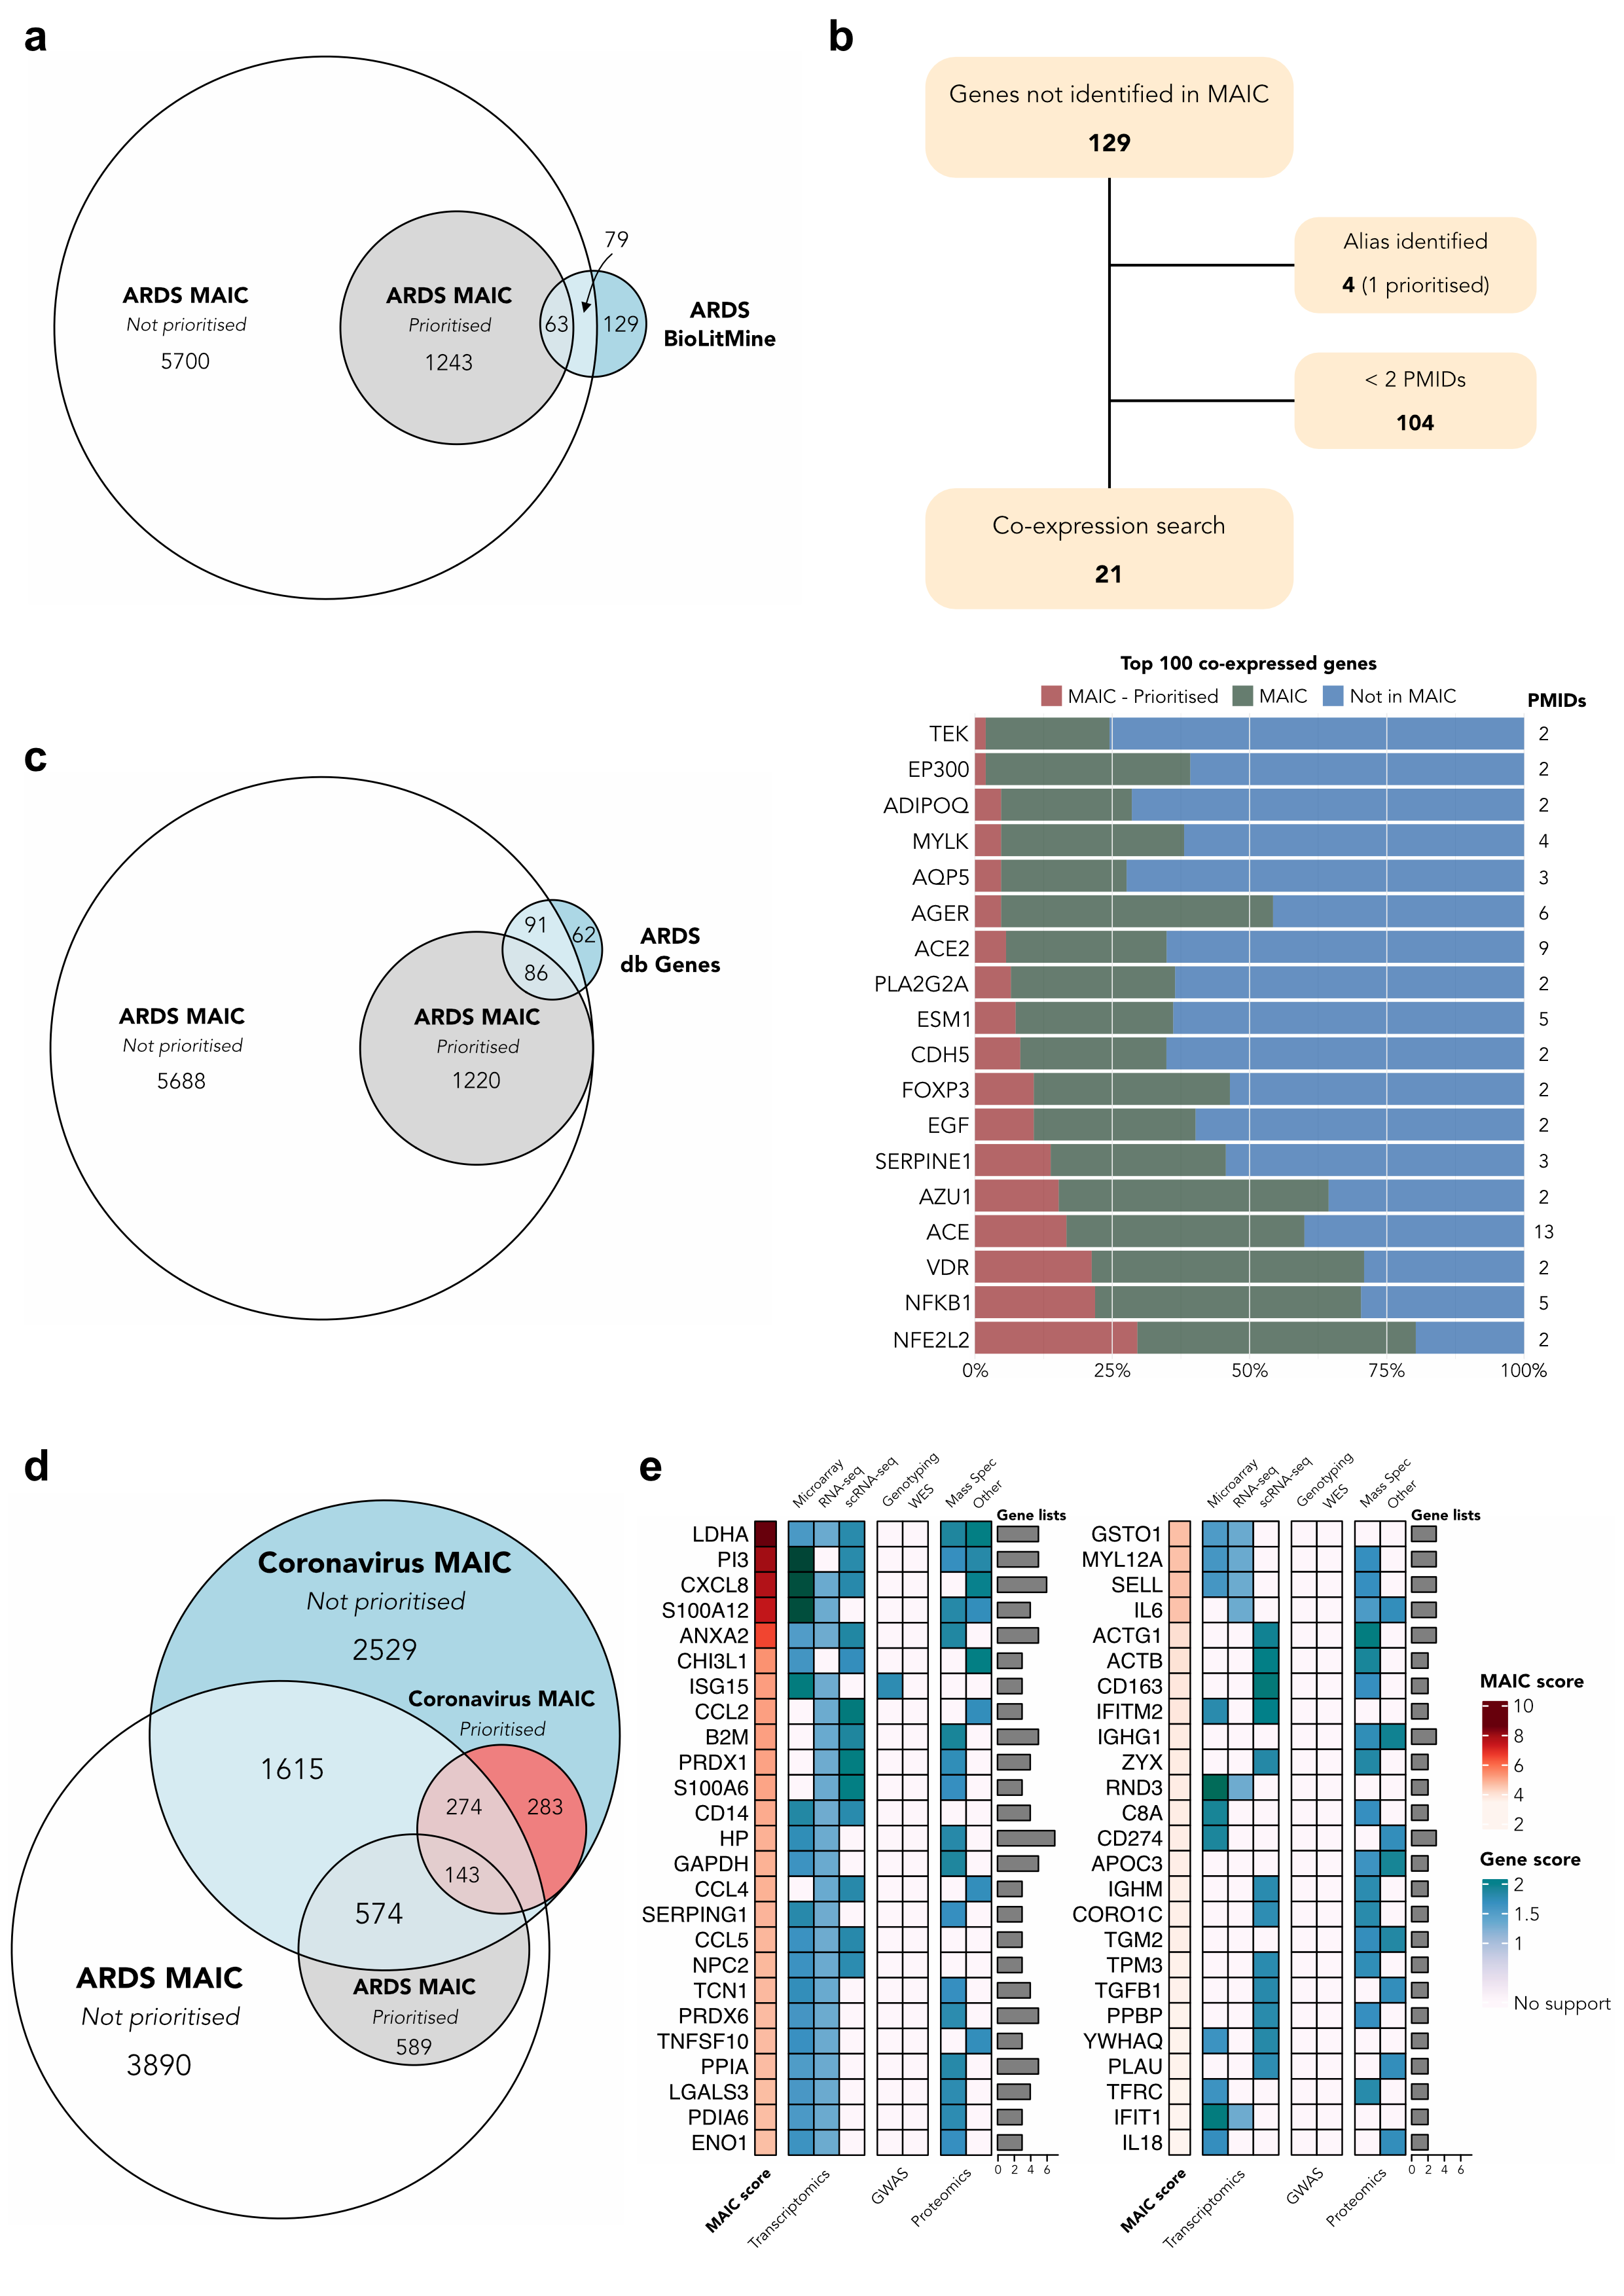
\includegraphics{../img/Supplementary_Figure_3.png}

}

\caption{\textbf{Tissue and cell-specific expression}. (a) Bar plot of
the tissue type in which genes are identified - all genes (n=7,085). (b)
Bar plot of the tissue type in which genes are identified - prioritised
genes (n=1,306). (c) Bar plot of the proportion of genes identified
solely in blood meeting mRNA expression thresholds in bulk lung tissue.
nTPM - normalised transcripts per million. (d) Heatmap of mRNA
expression in lung cell-types for genes identified in studies based on
airways sampling. (e) Heatmap of mRNA expression in blood cell-types for
genes identified solely in studies based on blood sampling. (f)
Manhatten plot of the top 20 cell types overenriched for expression of
genes identified by studies based on airways sampling. (g) Manhatten
plot of the top 20 cell types overenriched for expression of genes
identified by studies based on blood sampling.}

\end{figure}

\begin{figure}

{\centering 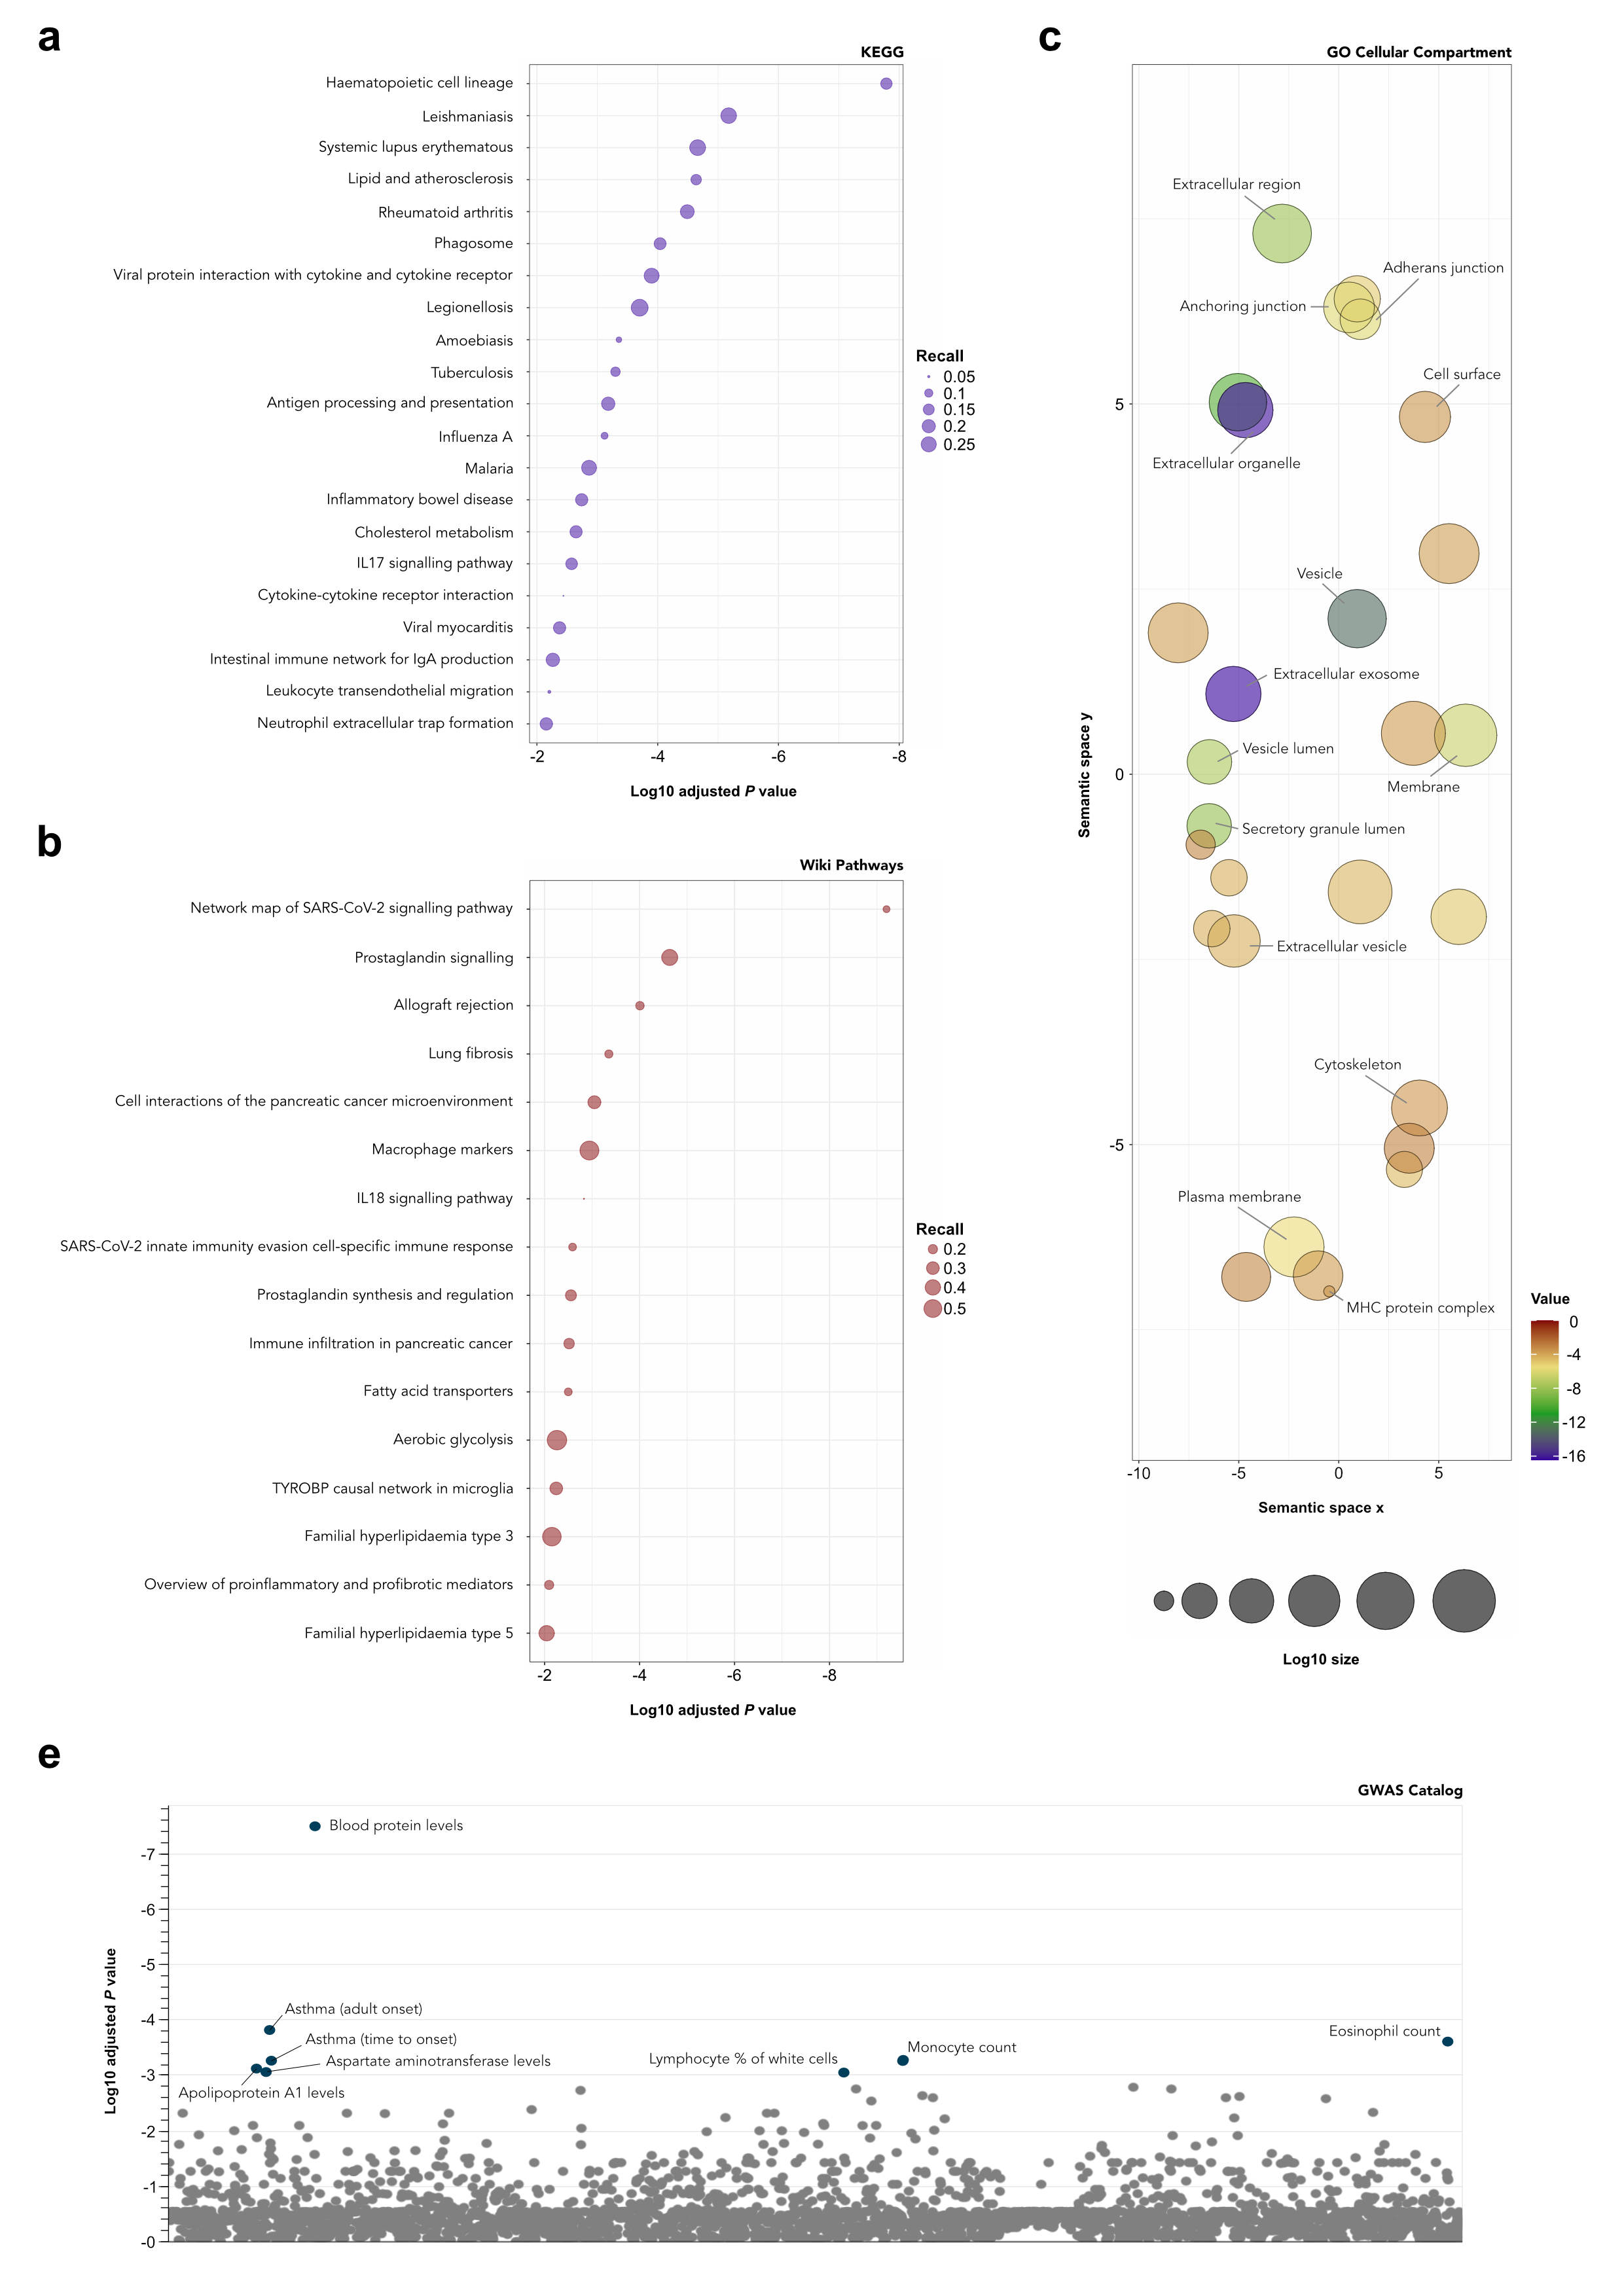
\includegraphics{../img/Supplementary_Figure_4.png}

}

\caption{\textbf{Functional enrichment}. (a) Significantly enriched KEGG
terms (\emph{P} \textless{} 0.01) for prioritised genes. Terms size
proportional to recall. (b) Significantly enriched WikiPathways terms
(\emph{P} \textless{} 0.01) for prioritised genes. Terms size
proportional to recall. (c) Scatter plot of the semantic similarity
between signficantly enriched GO cellular component terms for
prioritised genes (d) Manhatten plot of the overenrichment of
prioritised genes against the GWAS catolog.}

\end{figure}

\begin{figure}

{\centering 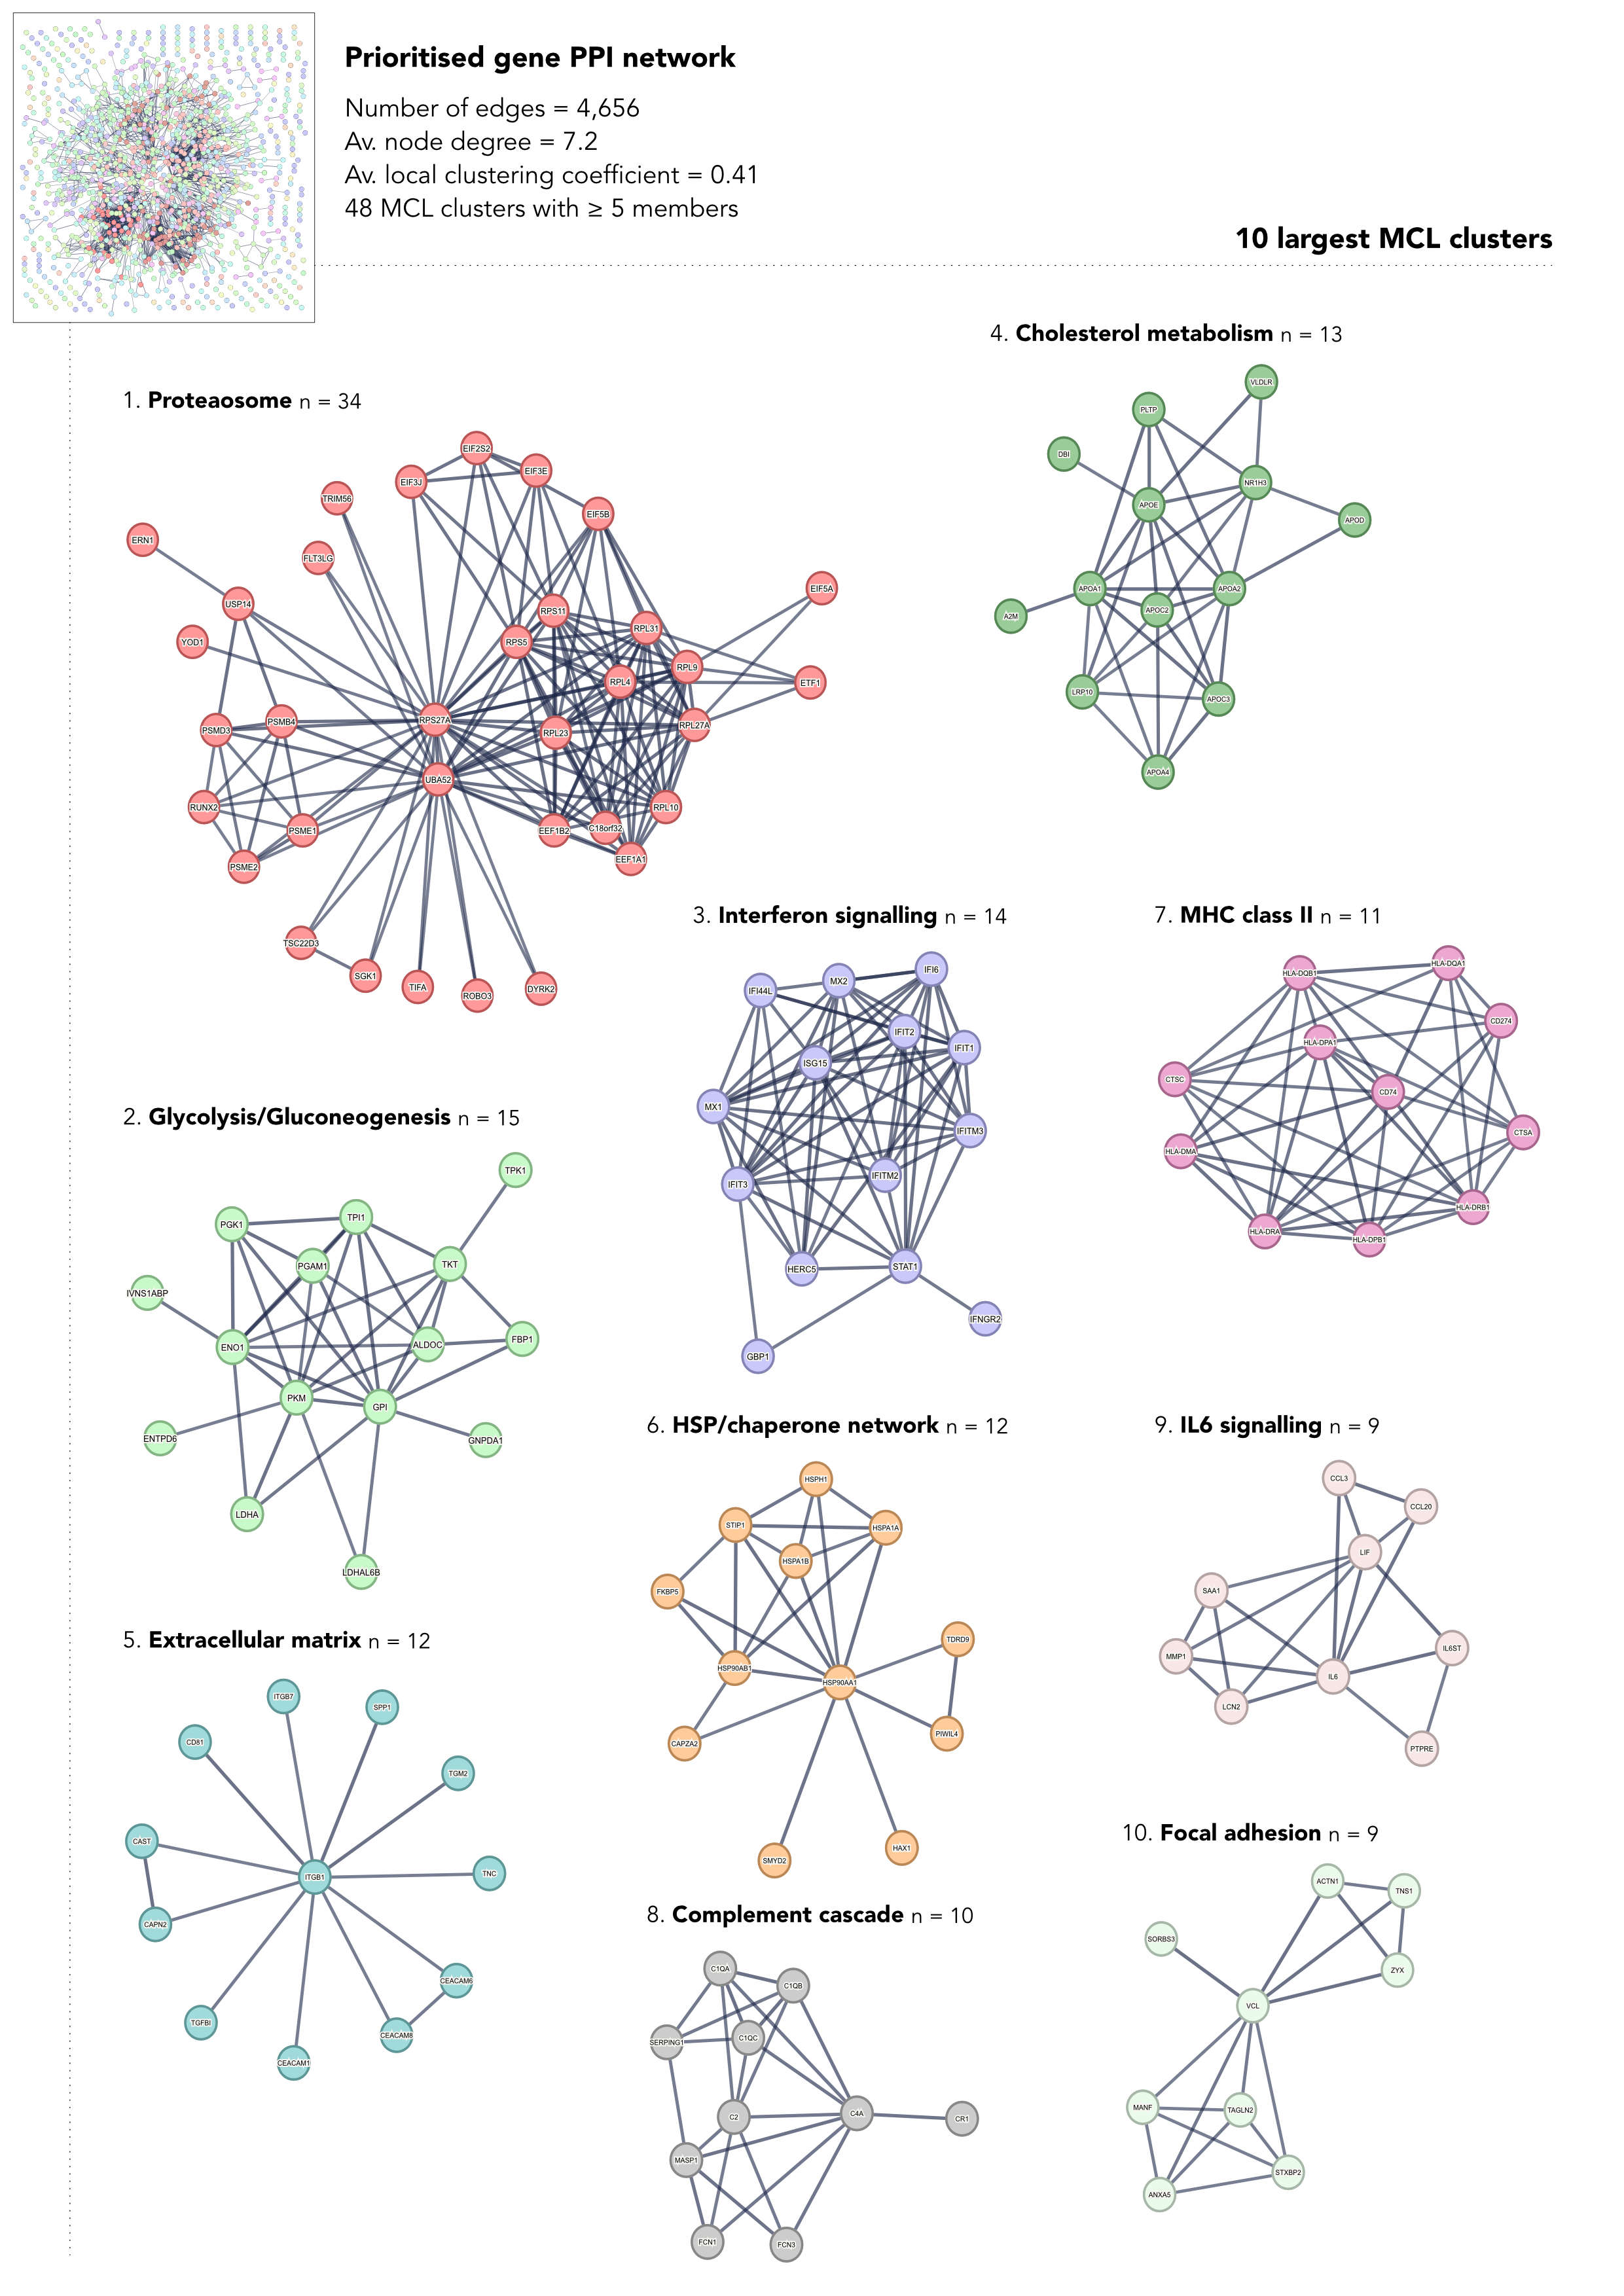
\includegraphics{../img/Supplementary_Figure_5.png}

}

\caption{\textbf{PPI clusters}. A protein-protein interaction network of
prioritsed genes and the 10 largest graph-based clusters. Functional
annotation by hand based on a concencus of enriched Reactome, KEGG,
WikiPathways, and GO Biological Process terms.}

\end{figure}

\begin{figure}

{\centering 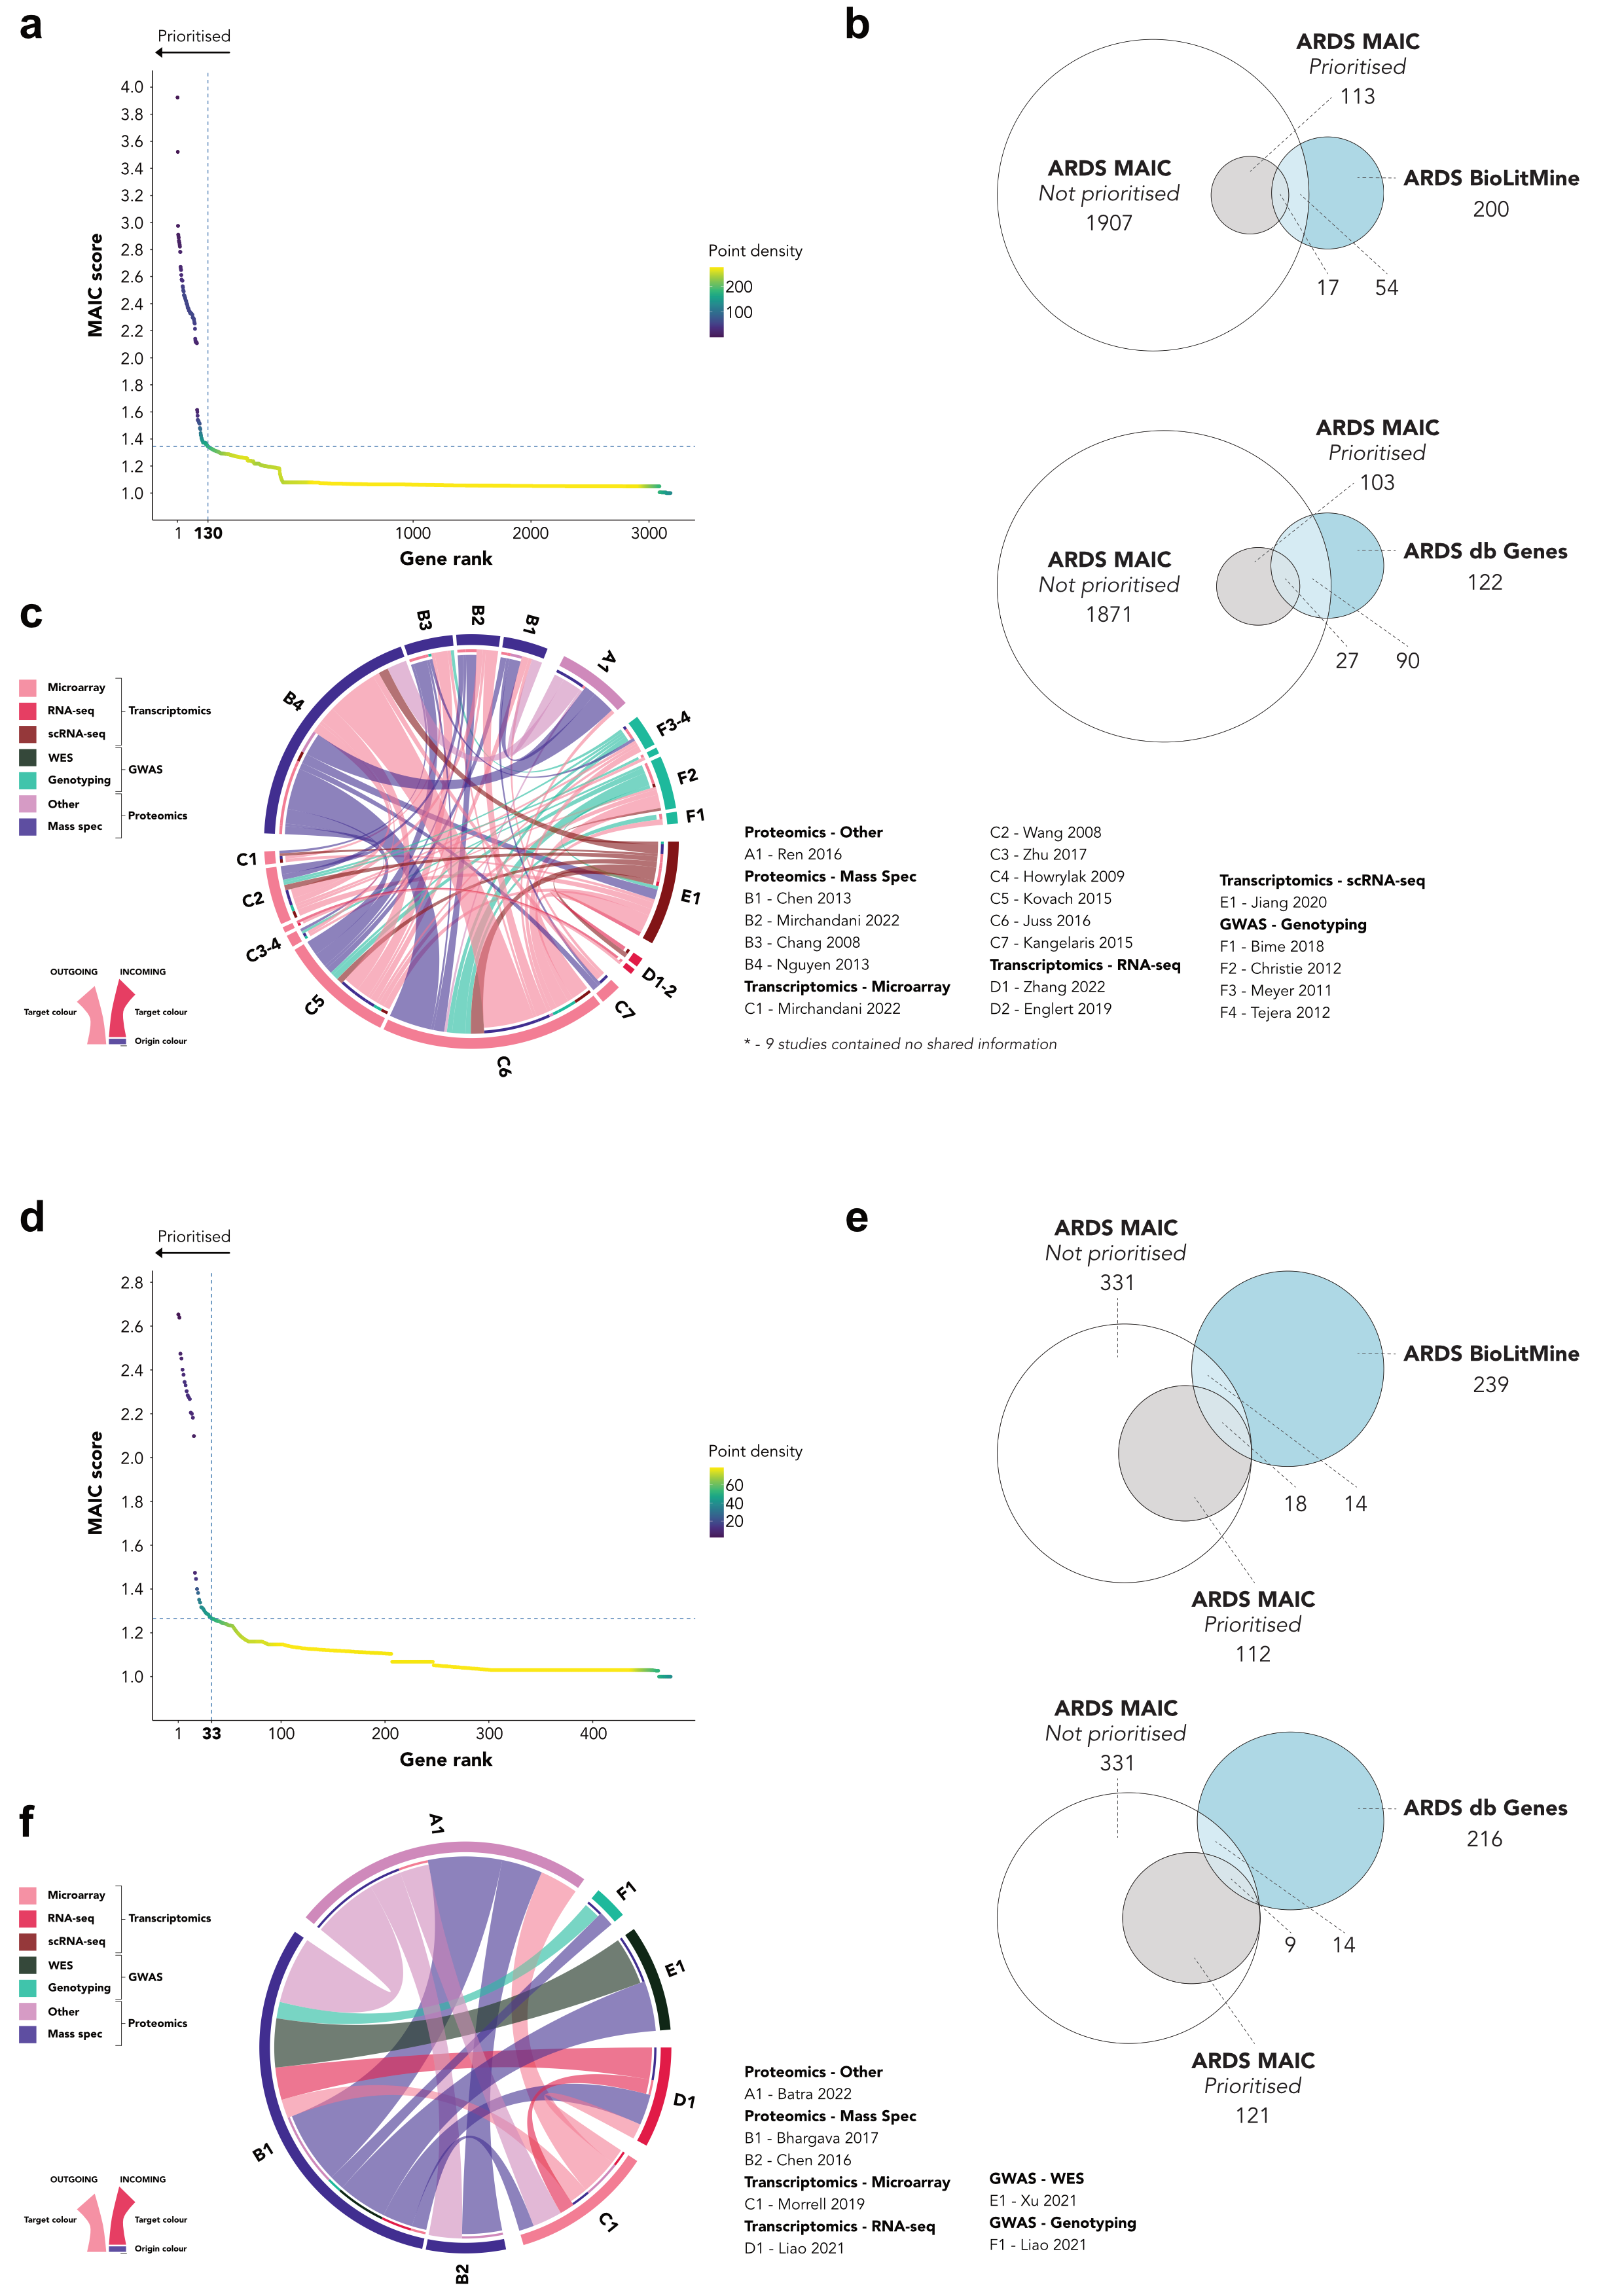
\includegraphics{../img/Supplementary_Figure_6.png}

}

\caption{\textbf{Details of MAIC on sub-groups}. (a) Gene prioritization
for the ARDS MAIC susceptibility sub-group using the Unit Invariant Knee
method. Intersection of lines identifies elbow point of best-fit curve.
130 genes in upper left quadrant were prioritied. (b) Eular diagrams of
gene overlap between the ARDS MAIC susceptibility sub-group and a
BioLitMine search using the ARDS MeSH term and the ARDS Database of
Genes. (c) Shared information content (IC) between susceptibility gene
lists. Links indicate absolute IC (sum of common gene scores) between
studies. (d) Gene prioritization for the ARDS MAIC survival sub-group
using the Unit Invariant Knee method. Intersection of lines identifies
elbow point of best-fit curve. 33 genes in upper left quadrant were
prioritied. (e) Eular diagrams of gene overlap between the ARDS MAIC
survival sub-group and a BioLitMine search using the ARDS MeSH term and
the ARDS Database of Genes. (f) Shared information content (IC) between
survival gene lists. Links indicate absolute IC (sum of common gene
scores) between studies.}

\end{figure}

\begin{figure}

{\centering 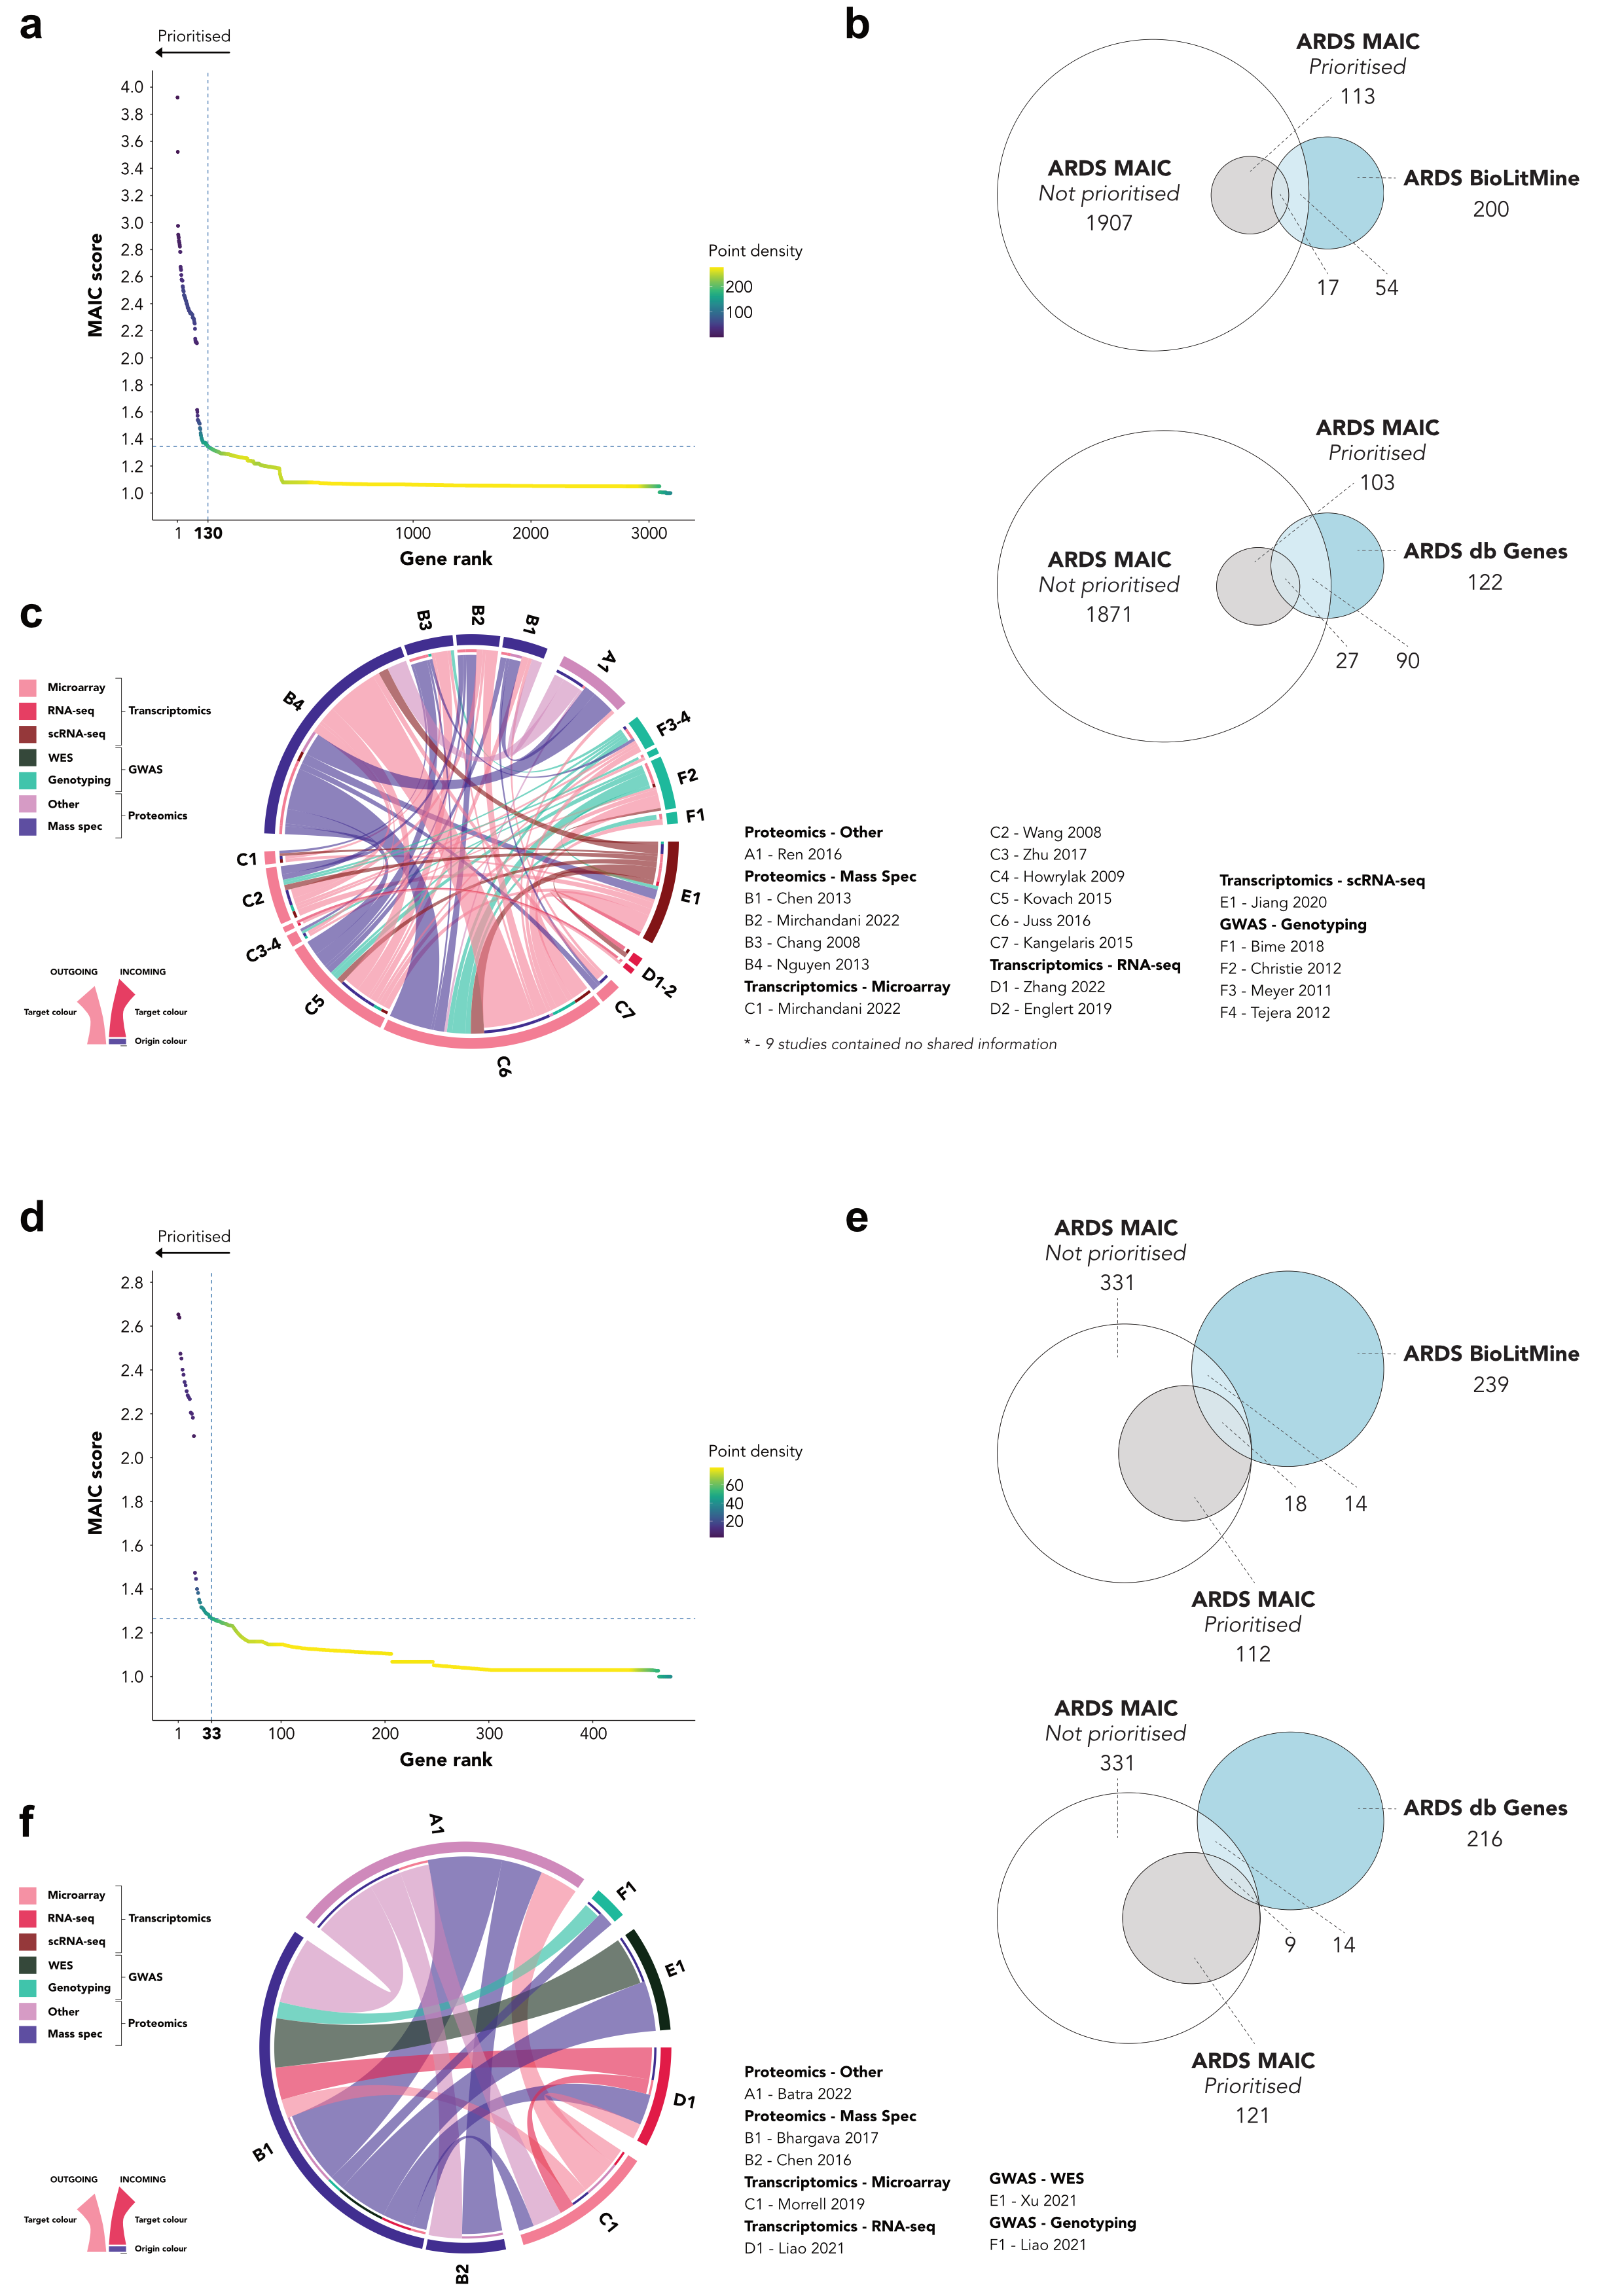
\includegraphics{../img/Supplementary_Figure_7.png}

}

\caption{\textbf{Sub-group functional enrichment}. (a) Significantly
enriched Reactome, WikiPathways, and KEGG terms (\emph{P} \textless{}
0.01) for prioritised genes in the susceptibility sub-group. Terms are
coloured by pathway and size is proportional to recall. (b) A
protein-protein interaction network of prioritsed genes in the
susceptibility cohort and graph-based clusters with ≥ 5 members. (c)
Significantly enriched Reactome, WikiPathways, and KEGG terms (\emph{P}
\textless{} 0.01) for prioritised genes in the survival sub-group. Terms
are coloured by pathway and size is proportional to recall. (d) A
protein-protein interaction network of prioritsed genes in the survival
cohort and graph-based clusters with ≥ 5 members.}

\end{figure}

\newpage

\textbf{Supplementary Table 1. Gene list information content and
contribution.}

\begin{longtable}[]{@{}
  >{\raggedright\arraybackslash}p{(\columnwidth - 10\tabcolsep) * \real{0.2818}}
  >{\raggedright\arraybackslash}p{(\columnwidth - 10\tabcolsep) * \real{0.1545}}
  >{\raggedright\arraybackslash}p{(\columnwidth - 10\tabcolsep) * \real{0.1273}}
  >{\raggedright\arraybackslash}p{(\columnwidth - 10\tabcolsep) * \real{0.1182}}
  >{\raggedright\arraybackslash}p{(\columnwidth - 10\tabcolsep) * \real{0.1455}}
  >{\raggedright\arraybackslash}p{(\columnwidth - 10\tabcolsep) * \real{0.1727}}@{}}
\toprule\noalign{}
\begin{minipage}[b]{\linewidth}\raggedright
\textbf{Study}
\end{minipage} & \begin{minipage}[b]{\linewidth}\raggedright
\textbf{Method}
\end{minipage} & \begin{minipage}[b]{\linewidth}\raggedright
\textbf{Category}
\end{minipage} & \begin{minipage}[b]{\linewidth}\raggedright
\textbf{N genes}
\end{minipage} & \begin{minipage}[b]{\linewidth}\raggedright
\textbf{rIC} (\%)
\end{minipage} & \begin{minipage}[b]{\linewidth}\raggedright
\textbf{rICtb} (\%)
\end{minipage} \\
\midrule\noalign{}
\endhead
\bottomrule\noalign{}
\endlastfoot
Sarma\textsuperscript{1} & Transcriptomics & RNA-seq & 4954 & 50.8 &
53.1 \\
Juss\textsuperscript{2} & Transcriptomics & Microarray & 1318 & 16 &
15.7 \\
Sarma\textsuperscript{1} & Transcriptomics & scRNA-seq & 706 & 9.8 &
10.3 \\
Nguyen\textsuperscript{3} & Proteomics & Mass Spec & 161 & 2.2 & 2.1 \\
Wang\textsuperscript{4} & Transcriptomics & Microarray & 137 & 1.9 &
1.9 \\
Bhargava\textsuperscript{5} & Proteomics & Mass Spec & 233 & 3.1 &
1.9 \\
Kovach\textsuperscript{6} & Transcriptomics & Microarray & 123 & 1.8 &
1.9 \\
Bhargava\textsuperscript{7} & Proteomics & Mass Spec & 144 & 1.9 &
1.8 \\
Morrell\textsuperscript{8} & Transcriptomics & Microarray & 155 & 1.9 &
1.7 \\
Christie\textsuperscript{9} & GWAS & Genotyping & 143 & 1.4 & 1.5 \\
Liao\textsuperscript{10} & GWAS & Genotyping & 67 & 0.7 & 0.8 \\
Sarma\textsuperscript{1} & Proteomics & Other & 60 & 0.8 & 0.7 \\
Jiang\textsuperscript{11} & Transcriptomics & scRNA-seq & 53 & 0.7 &
0.6 \\
Batra\textsuperscript{12} & Proteomics & Other & 39 & 0.6 & 0.6 \\
Bime\textsuperscript{13} & GWAS & Genotyping & 51 & 0.5 & 0.5 \\
Bos\textsuperscript{14} & Transcriptomics & Microarray & 53 & 0.7 &
0.5 \\
Chang\textsuperscript{15} & Proteomics & Mass Spec & 37 & 0.5 & 0.5 \\
Mirchandani\textsuperscript{16} & Transcriptomics & Microarray & 41 &
0.5 & 0.4 \\
Mirchandani\textsuperscript{16} & Proteomics & Mass Spec & 29 & 0.4 &
0.4 \\
Liao\textsuperscript{10} & Transcriptomics & RNA-seq & 43 & 0.4 & 0.4 \\
Dong\textsuperscript{17} & Proteomics & Mass Spec & 27 & 0.4 & 0.4 \\
Ren\textsuperscript{18} & Proteomics & Other & 17 & 0.3 & 0.3 \\
Tejera\textsuperscript{19} & GWAS & Genotyping & 19 & 0.3 & 0.3 \\
Howrylak\textsuperscript{20} & Transcriptomics & Microarray & 28 & 0.3 &
0.2 \\
Xu\textsuperscript{21} & GWAS & WES & 16 & 0.2 & 0.2 \\
Chen\textsuperscript{22} & Proteomics & Mass Spec & 16 & 0.2 & 0.2 \\
Zhang\textsuperscript{23} & Transcriptomics & RNA-seq & 20 & 0.2 &
0.2 \\
Kangelaris\textsuperscript{24} & Transcriptomics & Microarray & 15 & 0.2
& 0.2 \\
Meyer\textsuperscript{25} & GWAS & Genotyping & 10 & 0.1 & 0.1 \\
Martucci\textsuperscript{26} & Transcriptomics & Microarray & 13 & 0.1 &
0.1 \\
Zhu\textsuperscript{27} & Transcriptomics & Microarray & 14 & 0.1 &
0.1 \\
Englert\textsuperscript{28} & Transcriptomics & RNA-seq & 10 & 0.1 &
0.1 \\
Lu\textsuperscript{29} & Transcriptomics & Microarray & 12 & \textless{}
0.1 & \textless{} 0.1 \\
Scheller\textsuperscript{30} & Transcriptomics & RNA-seq & 9 &
\textless{} 0.1 & \textless{} 0.1 \\
Nick\textsuperscript{31} & Transcriptomics & Microarray & 4 &
\textless{} 0.1 & \textless{} 0.1 \\
Guillen-Guio\textsuperscript{32} & GWAS & Genotyping & 6 & \textless{}
0.1 & \textless{} 0.1 \\
Meyer\textsuperscript{33} & GWAS & Genotyping & 4 & \textless{} 0.1 &
\textless{} 0.1 \\
Dolinay\textsuperscript{34} & Transcriptomics & Microarray & 4 &
\textless{} 0.1 & \textless{} 0.1 \\
Chen\textsuperscript{35} & Proteomics & Mass Spec & 16 & \textless{} 0.1
& \textless{} 0.1 \\
Zhang\textsuperscript{36} & Transcriptomics & RNA-seq & 5 & \textless{}
0.1 & \textless{} 0.1 \\
Shortt\textsuperscript{37} & GWAS & WES & 3 & \textless{} 0.1 &
\textless{} 0.1 \\
Bowler\textsuperscript{38} & Proteomics & Mass Spec & 18 & \textless{}
0.1 & \textless{} 0.1 \\
Morrell\textsuperscript{39} & Transcriptomics & Microarray & 1 &
\textless{} 0.1 & \textless{} 0.1 \\
\end{longtable}

\begin{scriptsize}
Abbreviations: GWAS - Genome-wide association study; Mass Spec - Mass spectometry; rIC - Relative information content; rICtb - Relative information contribution; WES - Whole-exome sequencing.
\end{scriptsize}

\newpage

\textbf{Supplementary Table 2. ARDS MAIC prioritised genes found in
common by BioLitMine with \textgreater= 2 associated publications.}

\begin{longtable}[]{@{}
  >{\raggedright\arraybackslash}p{(\columnwidth - 6\tabcolsep) * \real{0.1128}}
  >{\raggedright\arraybackslash}p{(\columnwidth - 6\tabcolsep) * \real{0.1729}}
  >{\raggedright\arraybackslash}p{(\columnwidth - 6\tabcolsep) * \real{0.6015}}
  >{\raggedright\arraybackslash}p{(\columnwidth - 6\tabcolsep) * \real{0.1128}}@{}}
\toprule\noalign{}
\begin{minipage}[b]{\linewidth}\raggedright
\textbf{Gene}
\end{minipage} & \begin{minipage}[b]{\linewidth}\raggedright
\textbf{Publication count}
\end{minipage} & \begin{minipage}[b]{\linewidth}\raggedright
\textbf{PubMed IDs}
\end{minipage} & \begin{minipage}[b]{\linewidth}\raggedright
\textbf{MAIC rank}
\end{minipage} \\
\midrule\noalign{}
\endhead
\bottomrule\noalign{}
\endlastfoot
TGFB1 & 8 & 30395619, 29083412, 28188225, 27309347, 22034170, 20142324,
16100012, 12654639 & 225 \\
VEGFA & 8 & 24356493, 23542734, 21797753, 19543148, 19349383, 17289863,
15920019, 15741444 & 320 \\
IL10 & 8 & 32217834, 31936183, 30280795, 28432351, 22033829, 21138342,
18242340, 16585075 & 1268 \\
SFTPB & 6 & 21128671, 18679120, 16100012, 15190959, 14718442, 12490037 &
177 \\
IL17A & 6 & 34239039, 32795834, 32651218, 30655311, 26709006, 26002979 &
1294 \\
PI3 & 5 & 28187039, 24617927, 19251943, 19197381, 18203972 & 2 \\
CXCL8 & 5 & 22897124, 22080750, 21348591, 17498967, 14729508 & 3 \\
IL6 & 5 & 34757857, 33250487, 32826331, 31261506, 18593632 & 144 \\
TNF & 5 & 31261506, 22507624, 21784970, 17034639, 16135717 & 651 \\
NAMPT & 4 & 24821571, 24053186, 18486613, 17392604 & 58 \\
IL1RN & 4 & 30095747, 29943912, 23449693, 18838927 & 175 \\
SCGB1A1 & 4 & 32787812, 28548310, 18521628, 16215398 & 187 \\
NPPB & 4 & 28322314, 26359292, 21696613, 19830720 & 1239 \\
HGF & 3 & 18065658, 17702746, 11943656 & 343 \\
IL33 & 3 & 33936076, 31147742, 23000728 & 385 \\
CXCL10 & 3 & 31651197, 23542734, 23144331 & 671 \\
S100A12 & 2 & 26274928, 24887223 & 5 \\
MUC1 & 2 & 21418654, 17565019 & 69 \\
PLAU & 2 & 23064953, 17994220 & 244 \\
EPAS1 & 2 & 28613249, 25574837 & 425 \\
FASLG & 2 & 30385692, 12414525 & 503 \\
EDN1 & 2 & 27765761, 17875064 & 643 \\
AKT1 & 2 & 27607575, 15961723 & 950 \\
MMP8 & 2 & 24651234, 15187163 & 1223 \\
\end{longtable}

\newpage

\textbf{Supplementary Table 3. ARDS susceptibility gene list information
content and contribution.}

\begin{longtable}[]{@{}
  >{\raggedright\arraybackslash}p{(\columnwidth - 10\tabcolsep) * \real{0.2818}}
  >{\raggedright\arraybackslash}p{(\columnwidth - 10\tabcolsep) * \real{0.1545}}
  >{\raggedright\arraybackslash}p{(\columnwidth - 10\tabcolsep) * \real{0.1273}}
  >{\raggedright\arraybackslash}p{(\columnwidth - 10\tabcolsep) * \real{0.1182}}
  >{\raggedright\arraybackslash}p{(\columnwidth - 10\tabcolsep) * \real{0.1455}}
  >{\raggedright\arraybackslash}p{(\columnwidth - 10\tabcolsep) * \real{0.1727}}@{}}
\toprule\noalign{}
\begin{minipage}[b]{\linewidth}\raggedright
\textbf{Study}
\end{minipage} & \begin{minipage}[b]{\linewidth}\raggedright
\textbf{Method}
\end{minipage} & \begin{minipage}[b]{\linewidth}\raggedright
\textbf{Category}
\end{minipage} & \begin{minipage}[b]{\linewidth}\raggedright
\textbf{N genes}
\end{minipage} & \begin{minipage}[b]{\linewidth}\raggedright
\textbf{rIC} (\%)
\end{minipage} & \begin{minipage}[b]{\linewidth}\raggedright
\textbf{rICtb} (\%)
\end{minipage} \\
\midrule\noalign{}
\endhead
\bottomrule\noalign{}
\endlastfoot
Juss\textsuperscript{2} & Transcriptomics & Microarray & 1318 & 54.7 &
54.7 \\
Nguyen\textsuperscript{3} & Proteomics & Mass Spec & 161 & 8.1 & 7.7 \\
Christie\textsuperscript{9} & GWAS & Genotyping & 143 & 6 & 6.3 \\
Kovach\textsuperscript{6} & Transcriptomics & Microarray & 123 & 5.8 &
6.1 \\
Wang\textsuperscript{4} & Transcriptomics & Microarray & 137 & 5.8 &
6 \\
Jiang\textsuperscript{11} & Transcriptomics & scRNA-seq & 53 & 2.9 &
3 \\
Bime\textsuperscript{13} & GWAS & Genotyping & 51 & 2.2 & 2.3 \\
Mirchandani\textsuperscript{16} & Transcriptomics & Microarray & 41 &
1.7 & 1.6 \\
Chang\textsuperscript{15} & Proteomics & Mass Spec & 37 & 1.9 & 1.5 \\
Mirchandani\textsuperscript{16} & Proteomics & Mass Spec & 29 & 1.4 &
1.3 \\
Howrylak\textsuperscript{20} & Transcriptomics & Microarray & 28 & 1.2 &
1.3 \\
Ren\textsuperscript{18} & Proteomics & Other & 17 & 1 & 1.1 \\
Tejera\textsuperscript{19} & GWAS & Genotyping & 19 & 0.9 & 1 \\
Chen\textsuperscript{35} & Proteomics & Mass Spec & 16 & 0.9 & 0.9 \\
Zhang\textsuperscript{23} & Transcriptomics & RNA-seq & 20 & 0.8 &
0.9 \\
Zhu\textsuperscript{27} & Transcriptomics & Microarray & 14 & 0.6 &
0.6 \\
Kangelaris\textsuperscript{24} & Transcriptomics & Microarray & 15 & 0.7
& 0.6 \\
Englert\textsuperscript{28} & Transcriptomics & RNA-seq & 10 & 0.6 &
0.6 \\
Lu\textsuperscript{29} & Transcriptomics & Microarray & 12 & 0.5 &
0.5 \\
Meyer\textsuperscript{25} & GWAS & Genotyping & 10 & 0.4 & 0.4 \\
Bowler\textsuperscript{38} & Proteomics & Mass Spec & 18 & 0.9 & 0.4 \\
Scheller\textsuperscript{30} & Transcriptomics & RNA-seq & 9 & 0.4 &
0.3 \\
Guillen-Guio\textsuperscript{32} & GWAS & Genotyping & 6 & 0.2 & 0.2 \\
Zhang\textsuperscript{36} & Transcriptomics & RNA-seq & 5 & 0.2 & 0.2 \\
Dolinay\textsuperscript{34} & Transcriptomics & Microarray & 4 & 0.2 &
0.2 \\
Shortt\textsuperscript{37} & GWAS & WES & 3 & 0.1 & 0.1 \\
Meyer\textsuperscript{33} & GWAS & Genotyping & 4 & \textless{} 0.1 &
0.1 \\
Morrell\textsuperscript{39} & Transcriptomics & Microarray & 1 &
\textless{} 0.1 & \textless{} 0.1 \\
\end{longtable}

\begin{scriptsize}
Abbreviations: GWAS - Genome-wide association study; Mass Spec - Mass spectometry; rIC - Relative information content; rICtb - Relative information contribution; WES - Whole-exome sequencing.
\end{scriptsize}

\newpage

\textbf{Supplementary Table 4. ARDS survival/severity gene list
information content and contribution.}

\begin{longtable}[]{@{}
  >{\raggedright\arraybackslash}p{(\columnwidth - 10\tabcolsep) * \real{0.2818}}
  >{\raggedright\arraybackslash}p{(\columnwidth - 10\tabcolsep) * \real{0.1545}}
  >{\raggedright\arraybackslash}p{(\columnwidth - 10\tabcolsep) * \real{0.1273}}
  >{\raggedright\arraybackslash}p{(\columnwidth - 10\tabcolsep) * \real{0.1182}}
  >{\raggedright\arraybackslash}p{(\columnwidth - 10\tabcolsep) * \real{0.1455}}
  >{\raggedright\arraybackslash}p{(\columnwidth - 10\tabcolsep) * \real{0.1727}}@{}}
\toprule\noalign{}
\begin{minipage}[b]{\linewidth}\raggedright
\textbf{Study}
\end{minipage} & \begin{minipage}[b]{\linewidth}\raggedright
\textbf{Method}
\end{minipage} & \begin{minipage}[b]{\linewidth}\raggedright
\textbf{Category}
\end{minipage} & \begin{minipage}[b]{\linewidth}\raggedright
\textbf{N genes}
\end{minipage} & \begin{minipage}[b]{\linewidth}\raggedright
\textbf{rIC} (\%)
\end{minipage} & \begin{minipage}[b]{\linewidth}\raggedright
\textbf{rICtb} (\%)
\end{minipage} \\
\midrule\noalign{}
\endhead
\bottomrule\noalign{}
\endlastfoot
Bhargava\textsuperscript{7} & Proteomics & Mass Spec & 144 & 30.4 &
30.3 \\
Morrell\textsuperscript{8} & Transcriptomics & Microarray & 155 & 29.7 &
29.7 \\
Liao\textsuperscript{10} & GWAS & Genotyping & 67 & 12.9 & 13 \\
Batra\textsuperscript{12} & Proteomics & Other & 39 & 9.4 & 9.4 \\
Liao\textsuperscript{10} & Transcriptomics & RNA-seq & 43 & 8.5 & 8.5 \\
Xu\textsuperscript{21} & GWAS & WES & 16 & 3.5 & 3.5 \\
Chen\textsuperscript{22} & Proteomics & Mass Spec & 16 & 3.4 & 3.4 \\
Lu\textsuperscript{29} & Transcriptomics & Microarray & 12 & 2.2 &
2.2 \\
\end{longtable}

\begin{scriptsize}
Abbreviations: GWAS - Genome-wide association study; Mass Spec - Mass spectometry; rIC - Relative information content; rICtb - Relative information contribution; WES - Whole-exome sequencing.
\end{scriptsize}

\newpage

\hypertarget{supplementary-data}{%
\subsection{Supplementary Data}\label{supplementary-data}}

Supplementary Data Files 1-8

\newpage

\textbf{Supplementary Data File 1. Raw gene list input to MAIC}.

\url{https://github.com/JonathanEMillar/ards_maic_manuscript/Supplementary_Data_File_1.csv}

\textbf{Supplementary Data File 2. MAIC output - overall}.

\url{https://github.com/JonathanEMillar/ards_maic_manuscript/Supplementary_Data_File_2.csv}

\textbf{Supplementary Data File 3. BioLitMine and ARDS Database of Genes
results}.

\url{https://github.com/JonathanEMillar/ards_maic_manuscript/Supplementary_Data_File_3.csv}

\textbf{Supplementary Data File 4. MAIC output - susceptibility
sub-group}.

\url{https://github.com/JonathanEMillar/ards_maic_manuscript/Supplementary_Data_File_4.csv}

\textbf{Supplementary Data File 5. MAIC output - survival sub-group}.

\url{https://github.com/JonathanEMillar/ards_maic_manuscript/Supplementary_Data_File_5.csv}

\textbf{Supplementary Data File 6. Functional enrichment results -
overall}.

\url{https://github.com/JonathanEMillar/ards_maic_manuscript/Supplementary_Data_File_6.csv}

\textbf{Supplementary Data File 7. Functional enrichment results -
susceptibility sub-group}.

\url{https://github.com/JonathanEMillar/ards_maic_manuscript/Supplementary_Data_File_7.csv}

\textbf{Supplementary Data File 8. Functional enrichment results -
survival sub-group}.

\url{https://github.com/JonathanEMillar/ards_maic_manuscript/Supplementary_Data_File_8.csv}

\newpage

\hypertarget{references}{%
\subsection{References}\label{references}}

\hypertarget{refs}{}
\begin{CSLReferences}{0}{0}
\leavevmode\vadjust pre{\hypertarget{ref-Sarma2022}{}}%
\CSLLeftMargin{1. }%
\CSLRightInline{Sarma, A. \emph{et al.} Hyperinflammatory {ARDS} is
characterized by interferon-stimulated gene expression, t-cell
activation, and an altered metatranscriptome in tracheal aspirates.
\emph{bioRxiv} (2022).}

\leavevmode\vadjust pre{\hypertarget{ref-Juss2016}{}}%
\CSLLeftMargin{2. }%
\CSLRightInline{Juss, J. K. \emph{et al.} Acute respiratory distress
syndrome neutrophils have a distinct phenotype and are resistant to
phosphoinositide 3-kinase inhibition. \emph{Am. J. Respir. Crit. Care
Med.} \textbf{194}, 961--973 (2016).}

\leavevmode\vadjust pre{\hypertarget{ref-Nguyen2013}{}}%
\CSLLeftMargin{3. }%
\CSLRightInline{Nguyen, E. V. \emph{et al.} Proteomic profiling of
bronchoalveolar lavage fluid in critically ill patients with
ventilator-associated pneumonia. \emph{PLoS One} \textbf{8}, e58782
(2013).}

\leavevmode\vadjust pre{\hypertarget{ref-Wang2008}{}}%
\CSLLeftMargin{4. }%
\CSLRightInline{Wang, Z., Beach, D., Su, L., Zhai, R. \& Christiani, D.
C. A genome-wide expression analysis in blood identifies pre-elafin as a
biomarker in {ARDS}. \emph{Am. J. Respir. Cell Mol. Biol.} \textbf{38},
724--732 (2008).}

\leavevmode\vadjust pre{\hypertarget{ref-Bhargava2014}{}}%
\CSLLeftMargin{5. }%
\CSLRightInline{Bhargava, M. \emph{et al.} Proteomic profiles in acute
respiratory distress syndrome differentiates survivors from
non-survivors. \emph{PLoS One} \textbf{9}, e109713 (2014).}

\leavevmode\vadjust pre{\hypertarget{ref-Kovach2015}{}}%
\CSLLeftMargin{6. }%
\CSLRightInline{Kovach, M. A. \emph{et al.} Microarray analysis
identifies {IL-1} receptor type 2 as a novel candidate biomarker in
patients with acute respiratory distress syndrome. \emph{Respir. Res.}
\textbf{16}, 29 (2015).}

\leavevmode\vadjust pre{\hypertarget{ref-Bhargava2017}{}}%
\CSLLeftMargin{7. }%
\CSLRightInline{Bhargava, M. \emph{et al.} Bronchoalveolar lavage fluid
protein expression in acute respiratory distress syndrome provides
insights into pathways activated in subjects with different outcomes.
\emph{Sci. Rep.} \textbf{7}, 7464 (2017).}

\leavevmode\vadjust pre{\hypertarget{ref-Morrell2019}{}}%
\CSLLeftMargin{8. }%
\CSLRightInline{Morrell, E. D. \emph{et al.} Alveolar macrophage
transcriptional programs are associated with outcomes in acute
respiratory distress syndrome. \emph{Am. J. Respir. Crit. Care Med.}
\textbf{200}, 732--741 (2019).}

\leavevmode\vadjust pre{\hypertarget{ref-Christie2012}{}}%
\CSLLeftMargin{9. }%
\CSLRightInline{Christie, J. D. \emph{et al.} Genome wide association
identifies {PPFIA1} as a candidate gene for acute lung injury risk
following major trauma. \emph{PLoS One} \textbf{7}, e28268 (2012).}

\leavevmode\vadjust pre{\hypertarget{ref-Liao2021}{}}%
\CSLLeftMargin{10. }%
\CSLRightInline{Liao, S. Y. \emph{et al.} Identification of early and
intermediate biomarkers for {ARDS} mortality by multi-omic approaches.
\emph{Sci. Rep.} \textbf{11}, 18874 (2021).}

\leavevmode\vadjust pre{\hypertarget{ref-Jiang2020}{}}%
\CSLLeftMargin{11. }%
\CSLRightInline{Jiang, Y. \emph{et al.} Single cell {RNA} sequencing
identifies an early monocyte gene signature in acute respiratory
distress syndrome. \emph{JCI Insight} \textbf{5}, (2020).}

\leavevmode\vadjust pre{\hypertarget{ref-Batra2022}{}}%
\CSLLeftMargin{12. }%
\CSLRightInline{Batra, R. \emph{et al.} Multi-omic comparative analysis
of {COVID-19} and bacterial sepsis-induced {ARDS}. \emph{PLoS Pathog.}
\textbf{18}, e1010819 (2022).}

\leavevmode\vadjust pre{\hypertarget{ref-Bime2018}{}}%
\CSLLeftMargin{13. }%
\CSLRightInline{Bime, C. \emph{et al.} Genome-wide association study in
african americans with acute respiratory distress syndrome identifies
the selectin {P} ligand gene as a risk factor. \emph{Am. J. Respir.
Crit. Care Med.} \textbf{197}, 1421--1432 (2018).}

\leavevmode\vadjust pre{\hypertarget{ref-Bos2019}{}}%
\CSLLeftMargin{14. }%
\CSLRightInline{Bos, L. D. J. \emph{et al.} Understanding heterogeneity
in biologic phenotypes of acute respiratory distress syndrome by
leukocyte expression profiles. \emph{Am. J. Respir. Crit. Care Med.}
\textbf{200}, 42--50 (2019).}

\leavevmode\vadjust pre{\hypertarget{ref-Chang2008}{}}%
\CSLLeftMargin{15. }%
\CSLRightInline{Chang, D. W. \emph{et al.} Proteomic and computational
analysis of bronchoalveolar proteins during the course of the acute
respiratory distress syndrome. \emph{Am. J. Respir. Crit. Care Med.}
\textbf{178}, 701--709 (2008).}

\leavevmode\vadjust pre{\hypertarget{ref-Mirchandani2022}{}}%
\CSLLeftMargin{16. }%
\CSLRightInline{Mirchandani, A. S. \emph{et al.} Hypoxia shapes the
immune landscape in lung injury and promotes the persistence of
inflammation. \emph{Nat. Immunol.} \textbf{23}, 927--939 (2022).}

\leavevmode\vadjust pre{\hypertarget{ref-Dong2013}{}}%
\CSLLeftMargin{17. }%
\CSLRightInline{Dong, H. \emph{et al.} Comparative analysis of the
alveolar macrophage proteome in {ALI/ARDS} patients between the
exudative phase and recovery phase. \emph{BMC Immunol.} \textbf{14}, 25
(2013).}

\leavevmode\vadjust pre{\hypertarget{ref-Ren2016}{}}%
\CSLLeftMargin{18. }%
\CSLRightInline{Ren, S. \emph{et al.} Deleted in malignant brain tumors
1 protein is a potential biomarker of acute respiratory distress
syndrome induced by pneumonia. \emph{Biochem. Biophys. Res. Commun.}
\textbf{478}, 1344--1349 (2016).}

\leavevmode\vadjust pre{\hypertarget{ref-Tejera2012}{}}%
\CSLLeftMargin{19. }%
\CSLRightInline{Tejera, P. \emph{et al.} Distinct and replicable genetic
risk factors for acute respiratory distress syndrome of pulmonary or
extrapulmonary origin. \emph{J. Med. Genet.} \textbf{49}, 671--680
(2012).}

\leavevmode\vadjust pre{\hypertarget{ref-Howrylak2009}{}}%
\CSLLeftMargin{20. }%
\CSLRightInline{Howrylak, J. A. \emph{et al.} Discovery of the gene
signature for acute lung injury in patients with sepsis. \emph{Physiol.
Genomics} \textbf{37}, 133--139 (2009).}

\leavevmode\vadjust pre{\hypertarget{ref-Xu2021}{}}%
\CSLLeftMargin{21. }%
\CSLRightInline{Xu, J.-Y. \emph{et al.} Nucleotide polymorphism in
{ARDS} outcome: A whole exome sequencing association study. \emph{Ann.
Transl. Med.} \textbf{9}, 780 (2021).}

\leavevmode\vadjust pre{\hypertarget{ref-Chen2016}{}}%
\CSLLeftMargin{22. }%
\CSLRightInline{Chen, C., Shi, L., Li, Y., Wang, X. \& Yang, S.
Disease-specific dynamic biomarkers selected by integrating inflammatory
mediators with clinical informatics in {ARDS} patients with severe
pneumonia. \emph{Cell Biol. Toxicol.} \textbf{32}, 169--184 (2016).}

\leavevmode\vadjust pre{\hypertarget{ref-Zhang2022}{}}%
\CSLLeftMargin{23. }%
\CSLRightInline{Zhang, C. \emph{et al.} Differential expression profile
of plasma exosomal {microRNAs} in acute type a aortic dissection with
acute lung injury. \emph{Sci. Rep.} \textbf{12}, 11667 (2022).}

\leavevmode\vadjust pre{\hypertarget{ref-Kangelaris2015}{}}%
\CSLLeftMargin{24. }%
\CSLRightInline{Kangelaris, K. N. \emph{et al.} Increased expression of
neutrophil-related genes in patients with early sepsis-induced {ARDS}.
\emph{Am. J. Physiol. Lung Cell. Mol. Physiol.} \textbf{308}, L1102--13
(2015).}

\leavevmode\vadjust pre{\hypertarget{ref-Meyer2013}{}}%
\CSLLeftMargin{25. }%
\CSLRightInline{Meyer, N. J. \emph{et al.} {IL1RN} coding variant is
associated with lower risk of acute respiratory distress syndrome and
increased plasma {IL-1} receptor antagonist. \emph{Am. J. Respir. Crit.
Care Med.} \textbf{187}, 950--959 (2013).}

\leavevmode\vadjust pre{\hypertarget{ref-Martucci2020}{}}%
\CSLLeftMargin{26. }%
\CSLRightInline{Martucci, G. \emph{et al.} Identification of a
circulating {miRNA} signature to stratify acute respiratory distress
syndrome patients. \emph{J. Pers. Med.} \textbf{11}, 15 (2020).}

\leavevmode\vadjust pre{\hypertarget{ref-Zhu2017}{}}%
\CSLLeftMargin{27. }%
\CSLRightInline{Zhu, Z. \emph{et al.} Whole blood {microRNA} markers are
associated with acute respiratory distress syndrome. \emph{Intensive
Care Med. Exp.} \textbf{5}, 38 (2017).}

\leavevmode\vadjust pre{\hypertarget{ref-Englert2019}{}}%
\CSLLeftMargin{28. }%
\CSLRightInline{Englert, J. A. \emph{et al.} Whole blood {RNA}
sequencing reveals a unique transcriptomic profile in patients with
{ARDS} following hematopoietic stem cell transplantation. \emph{Respir.
Res.} \textbf{20}, 15 (2019).}

\leavevmode\vadjust pre{\hypertarget{ref-Lu2017}{}}%
\CSLLeftMargin{29. }%
\CSLRightInline{Lu, X.-G. \emph{et al.} Circulating {miRNAs} as
biomarkers for severe acute pancreatitis associated with acute lung
injury. \emph{World J. Gastroenterol.} \textbf{23}, 7440--7449 (2017).}

\leavevmode\vadjust pre{\hypertarget{ref-Scheller2019}{}}%
\CSLLeftMargin{30. }%
\CSLRightInline{Scheller, N. \emph{et al.} Proviral {MicroRNAs} detected
in extracellular vesicles from bronchoalveolar lavage fluid of patients
with influenza virus-induced acute respiratory distress syndrome.
\emph{J. Infect. Dis.} \textbf{219}, 540--543 (2019).}

\leavevmode\vadjust pre{\hypertarget{ref-Nick2016}{}}%
\CSLLeftMargin{31. }%
\CSLRightInline{Nick, J. A. \emph{et al.} Extremes of
interferon-stimulated gene expression associate with worse outcomes in
the acute respiratory distress syndrome. \emph{PLoS One} \textbf{11},
e0162490 (2016).}

\leavevmode\vadjust pre{\hypertarget{ref-GuillenGuio2020}{}}%
\CSLLeftMargin{32. }%
\CSLRightInline{Guillen-Guio, B. \emph{et al.} Sepsis-associated acute
respiratory distress syndrome in individuals of european ancestry: A
genome-wide association study. \emph{Lancet Respir. Med.} \textbf{8},
258--266 (2020).}

\leavevmode\vadjust pre{\hypertarget{ref-Meyer2011}{}}%
\CSLLeftMargin{33. }%
\CSLRightInline{Meyer, N. J. \emph{et al.} {ANGPT2} genetic variant is
associated with trauma-associated acute lung injury and altered plasma
angiopoietin-2 isoform ratio. \emph{Am. J. Respir. Crit. Care Med.}
\textbf{183}, 1344--1353 (2011).}

\leavevmode\vadjust pre{\hypertarget{ref-Dolinay2012}{}}%
\CSLLeftMargin{34. }%
\CSLRightInline{Dolinay, T. \emph{et al.} Inflammasome-regulated
cytokines are critical mediators of acute lung injury. \emph{Am. J.
Respir. Crit. Care Med.} \textbf{185}, 1225--1234 (2012).}

\leavevmode\vadjust pre{\hypertarget{ref-Chen2013}{}}%
\CSLLeftMargin{35. }%
\CSLRightInline{Chen, X., Shan, Q., Jiang, L., Zhu, B. \& Xi, X.
Quantitative proteomic analysis by {iTRAQ} for identification of
candidate biomarkers in plasma from acute respiratory distress syndrome
patients. \emph{Biochem. Biophys. Res. Commun.} \textbf{441}, 1--6
(2013).}

\leavevmode\vadjust pre{\hypertarget{ref-Zhang2021}{}}%
\CSLLeftMargin{36. }%
\CSLRightInline{Zhang, S. \emph{et al.} miR-584 and miR-146 are
candidate biomarkers for acute respiratory distress syndrome. \emph{Exp.
Ther. Med.} \textbf{21}, 445 (2021).}

\leavevmode\vadjust pre{\hypertarget{ref-Shortt2014}{}}%
\CSLLeftMargin{37. }%
\CSLRightInline{Shortt, K. \emph{et al.} Identification of novel single
nucleotide polymorphisms associated with acute respiratory distress
syndrome by exome-seq. \emph{PLoS One} \textbf{9}, e111953 (2014).}

\leavevmode\vadjust pre{\hypertarget{ref-Bowler2004}{}}%
\CSLLeftMargin{38. }%
\CSLRightInline{Bowler, R. P. \emph{et al.} Proteomic analysis of
pulmonary edema fluid and plasma in patients with acute lung injury.
\emph{Am. J. Physiol. Lung Cell. Mol. Physiol.} \textbf{286}, L1095--104
(2004).}

\leavevmode\vadjust pre{\hypertarget{ref-Morrell2018}{}}%
\CSLLeftMargin{39. }%
\CSLRightInline{Morrell, E. D. \emph{et al.} Cytometry {TOF} identifies
alveolar macrophage subtypes in acute respiratory distress syndrome.
\emph{JCI Insight} \textbf{3}, (2018).}

\end{CSLReferences}



\end{document}
